\documentclass[a4paper,10pt,oneside,onecolumn]{book}

\setlength{\textwidth}{160mm}
\setlength{\textheight}{260mm}
\setlength{\oddsidemargin}{-0cm}
\setlength{\evensidemargin}{28mm}
\setlength{\topmargin}{2cm}

\usepackage[
top    = 3.75cm,
bottom = 2.50cm,
left   = 3.00cm,
right  = 2.50cm]{geometry}


%\usepackage[spanish]{babel}
%\usepackage{tikz}
%\usetikzlibrary{babel}
%\usepackage[spanish]{babel}

\usepackage[utf8]{inputenc}
\usepackage[T1]{fontenc}
\usepackage{textcomp}
\usepackage{lmodern}

\usepackage{amsmath,amssymb}
\usepackage{latexsym}
\usepackage{makebox}
\usepackage{fancyhdr}

\usepackage{float}
\usepackage{graphicx}
\usepackage{epstopdf}
\usepackage{epsfig} 

\usepackage{amsfonts}
\usepackage{graphics}
\usepackage{color}
\usepackage{multicol} 

\usepackage{pstricks}
\usepackage{pst-node}
\usepackage{pst-plot}

\title{
Análisis Matemático\\
\textbf{Teoria}}
\author{
Facundo Beltramo\\
contacto: fexbef[at]gmail[dot]com
}
\date{Fecha: xx de xx del 201x}


\pagestyle{fancy} 
%\lhead{Consejos para comprar una Computadora}
%\rhead{lalala}
\renewcommand{\headrulewidth}{0.4pt} % grosor de la línea de la cabecera

\setcounter{secnumdepth}{3} % para que ponga 1.1.1.1 en subsubsecciones...
\setcounter{tocdepth}{4} % para que añada las subsubsecciones y párrafos en el indice...

\begin{document}
\maketitle

\tableofcontents % indice de contenidos


%\renewcommand{\thepage}{\arabic{page}}
%\setcounter{page}{1}


\chapter{Funciones Reales}\label{cap.Funcines}
\pagenumbering{arabic} % para empezar la numeración con números

\section{Definición de Función}
Una Función Real de una variable Real es una regla o una ley que asigna a cada uno de los elementos de un cierto subconjunto de los $\mathbb{R}$ un único elemento $\mathbb{R}$.

Notación:
$$f: D \in \mathbb{R} \longrightarrow C \in \mathbb{R}$$ 
$$x \longrightarrow y = f(x)$$
$f$ toma un $x$ de $D$ y devuelve un $y$ perteneciente a $C$. Donde $D$ es el dominio de la función, $y=f(x)$ es el valor de $f$ en $x$ y $C$ es el codominio de la función. 
\subsection{Definicion: Dominio}
Llamaremos Conjunto de Partida o Dominio de $f$, a el conjunto de todos los posibles valores de ingreso que la función acepta y lo notamos Dom$f$.
\subsection{Definición: Codominio}
Llamaremos Conjunto de Llegada o Codominio de $f$, a el conjunto de todos los valores de salida de una función y lo notamos Cod$f$.
\subsection{Definición: Imagen}
Llamaremos recorrido o imagen de $f$, al conjunto Im$f=$\{$f(x)/x \in $Dom$f$\}
\section{Primeras Funciones con nombre}
Existen ciertas funciones que suelen encontrarse con frecuencia en variados problemas y para poder hacer mejor referencia a ellas se les dio nombre.
\subsection{Función Constante}
\hfill
\begin{minipage}{.45\textwidth}
$$f:\mathbb{R} \longrightarrow \mathbb{R}$$
$$x \longrightarrow f(x)= k, k \in \mathbb{R}$$\\
Dom$f = \mathbb{R}$\\
Cod$f = \mathbb{R}$\\
Im$f = \mathbb{R}$\\
\end{minipage}
\hfill
\begin{minipage}{.45\textwidth}
\begin{center}
Grafica de $f(x)= k$
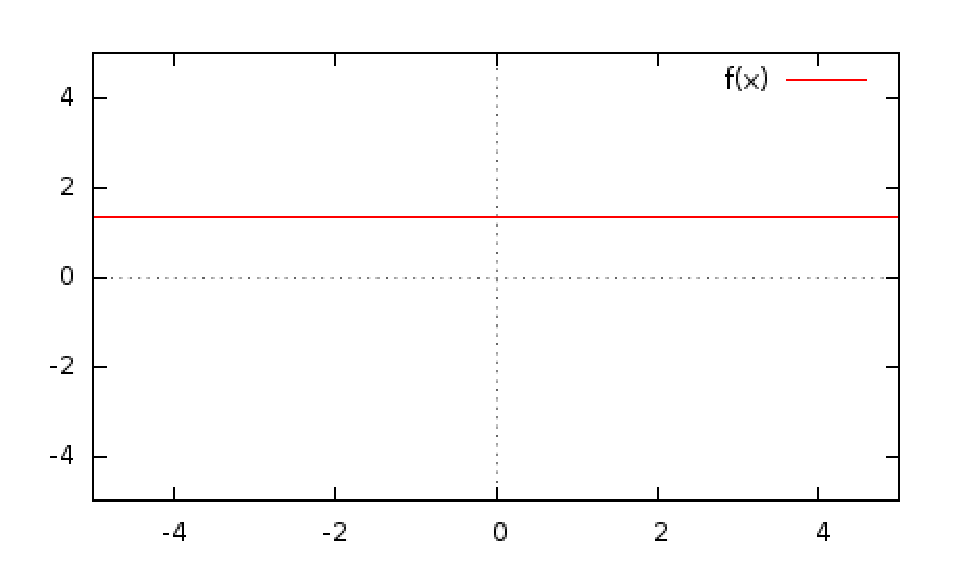
\includegraphics[height=4cm,width=6cm]{fconst.eps} 
\end{center}
\end{minipage}
\hfill
\subsection{Funcion Identidad}
\hfill
\begin{minipage}{.45\textwidth}
$$f:\mathbb{R} \longrightarrow \mathbb{R}$$
$$x \longrightarrow f(x)= x$$\\
Dom$f = \mathbb{R}$\\
Cod$f = \mathbb{R}$\\
Im$f = \mathbb{R}$\\
\end{minipage}
\hfill
\begin{minipage}{.45\textwidth}
\begin{center}
Grafica de $f(x)= x$
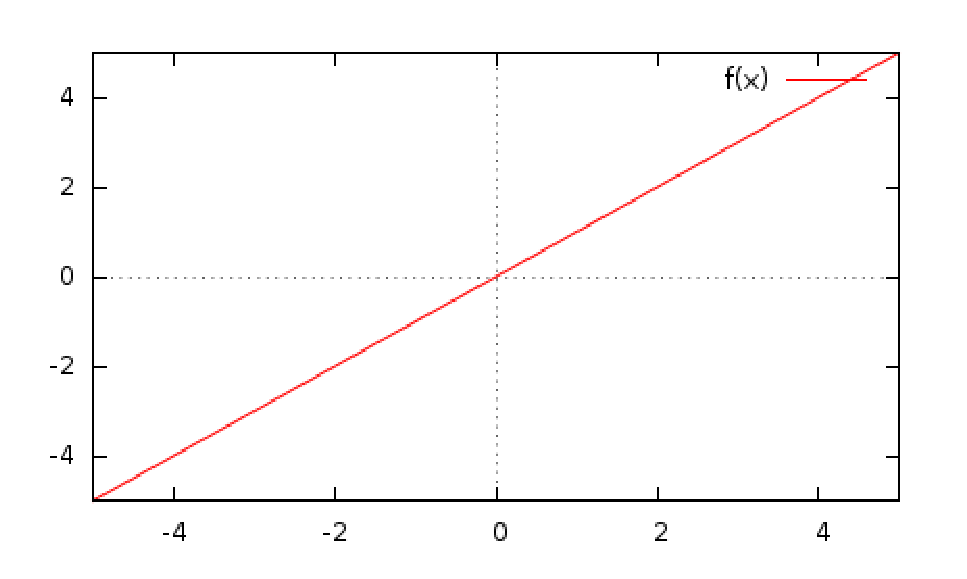
\includegraphics[height=4cm,width=6cm]{fid.eps} 
\end{center}
\end{minipage}
\hfill
\subsection{Función Valor Absoluto}
\hfill
\begin{minipage}{.45\textwidth}
\hfill
\begin{minipage}{.45\textwidth}
$$f:\mathbb{R} \longrightarrow \mathbb{R}$$
$$x \longrightarrow f(x)= |x|$$\\
$$|x|= \left\{
\begin{array}{c l}
  x & x>0 \\
  -x & x<0
\end{array}
\right.$$
\end{minipage}
\hfill
\begin{minipage}{.45\textwidth}
\begin{center}
Dom$f = \mathbb{R}$\\
Cod$f = \mathbb{R}$\\
Im$f = \mathbb{R} ^{+} _{0}$\\
\end{center}
\end{minipage}
\hfill
\end{minipage}
\hfill
\begin{minipage}{.45\textwidth}
\begin{center}
Grafica de $f(x)= |x|$
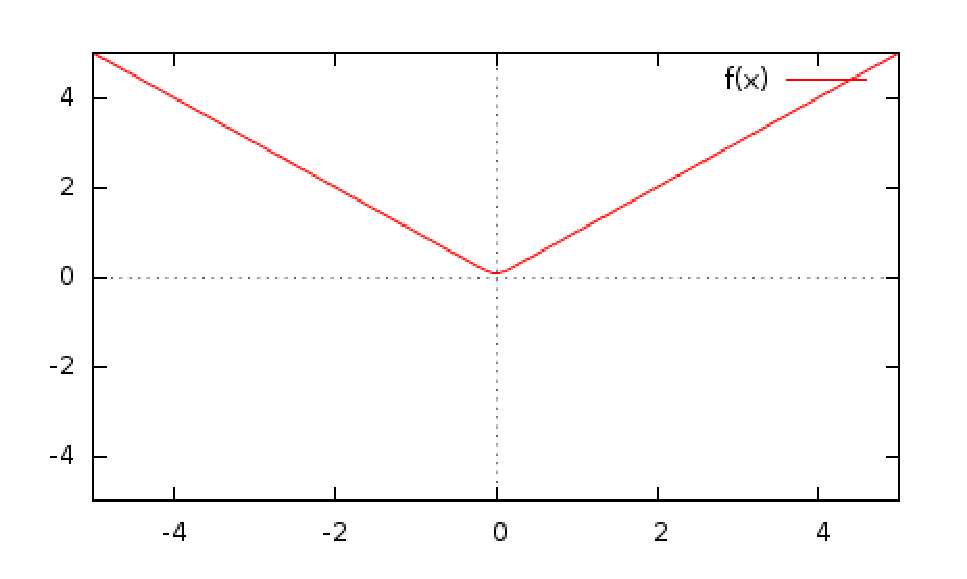
\includegraphics[height=4cm,width=6cm]{fabs.eps} 
\end{center}
\end{minipage}
\hfill
\subsubsection{Propiedades del Valor Absoluto}

• $|x|=|-x|$ o bien $f(x)=f(-x)$ (es una función par)\\

• $f(f(x))=\left\{
\begin{array}{c l}
  f(x) & f(x)>0 \\
  -f(x) & f(x)<0 \longrightarrow$ no se da nunca $
\end{array}
\right. \Rightarrow ||x|| = |x|$\\

• $f(x+y) \leqslant f(x)+f(y)$ es decir $|x+y| \leqslant |x|+|y|$ (conocida como Desigualdad Triangular)\\

• $f(x) = \sqrt{x^{2}}$ es decir $|x|=\sqrt{x^{2}}$

\section{Álgebra de funciones}Sean: $f: A \in \mathbb{R} \longrightarrow \mathbb{R}$, y
			$g: B \in \mathbb{R} \longrightarrow \mathbb{R}$, definiremos las siguientes funciones:
\subsection{Función Suma}
$$f+g:A \cap B \longrightarrow \mathbb{R}$$
$$x \longrightarrow (f+g)(x)= f(x)+g(x)$$
\subsection{Función Diferencia}
$$f-g:A \cap B \longrightarrow \mathbb{R}$$
$$x \longrightarrow (f-g)(x)= f(x)-g(x)$$
\subsection{Función Producto}
\begin{center}
$f$ x $g:A \cap B \longrightarrow \mathbb{R}$\\
$x \longrightarrow (f$ x $g)(x)= f(x)$ x $g(x)$
\end{center}
\subsection{Función Cociente}
\begin{center}
$f/g:$ \{$x \in A \cap B / g(x)\neq0$\}$ \longrightarrow \mathbb{R}$\\
$x \longrightarrow (f/g)(x)= \frac{f(x)}{g(x)}$
\end{center}

\section{Gráfica de función}
\subsection{Definicion}
Sea $f$ una función real, llamamos gráfica o grafo de $f$ al lugar geométrico de los puntos $(x,y)$ del plano tale que $x \in $ Dom$f$ e $y=f(x)$ es decir, lo notamos:\\
\begin{center}
Gr$f=$\{$(x,y) \in \mathbb{R} ^{2} / x \in $ Dom$f \wedge y=f(x)$\}
\end{center}
\subsection{Función Parte Entera}
\begin{center}
$f: \mathbb{R} \longrightarrow \mathbb{N}$\\
$x \longrightarrow f(x) = \lfloor x \rfloor = n \rightarrow$ ``Mayor entero que no supera a $x$''
\end{center}
\hfill
\begin{minipage}{.45\textwidth}
\begin{center}
otra definicion
\end{center}
$$\lfloor x \rfloor=\left\{
\begin{array}{c l}a
  -n & -n\leqslant x < -n+1 \\
  . & . \\
  . & . \\
  -2 & -2 \leqslant x < -2+1 \\
  -1 & -1 \leqslant x < -1+1 \\
  0 & 0 \leqslant x < 0+1 \\
  1 & 1 \leqslant x < 1+1 \\
  2 & 2 \leqslant x < 2+1 \\
  . & . \\
  . & . \\
  n & n \leqslant x < n+1 \\
\end{array}
\right.$$

\end{minipage}
\hfill
\begin{minipage}{.45\textwidth}
\begin{center}
Grafica de $f(x)= \lfloor x \rfloor$
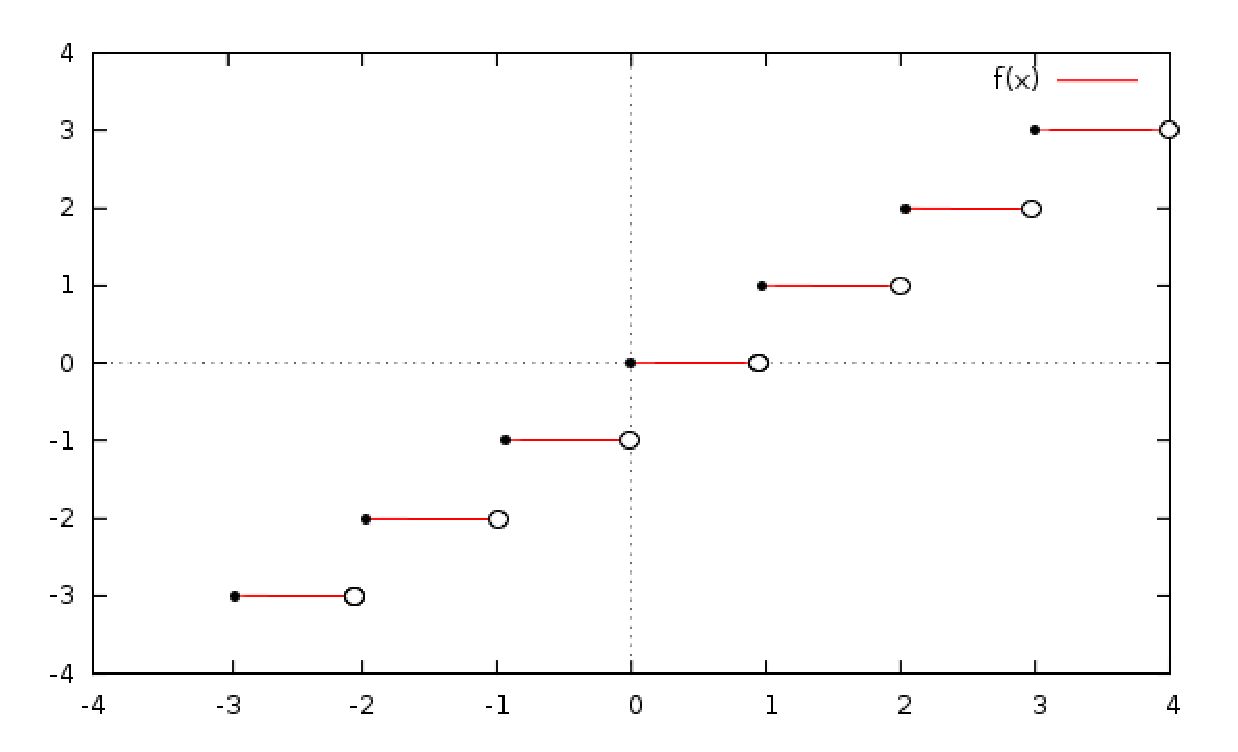
\includegraphics[height=4cm,width=6cm]{fpartent.eps} 
Dom$f = \mathbb{R}$, Cod$f = \mathbb{N}$, Im$f = \mathbb{N}$\\
\end{center}
\end{minipage}
\hfill
\\\\

La gráfica corresponde a: Gr$f=$\{$(x,f(x))/ x \in $Dom$f$\}

\subsection{Función Mantisa}
\hfill
\begin{minipage}{.45\textwidth}
$$f: \mathbb{R} \longrightarrow \mathbb{R}$$
$$x \longrightarrow f(x) = x - \lfloor x \rfloor = m(x)$$
\begin{center}
Sea $x \in \mathbb{R}$\\
$\lfloor x \rfloor \leqslant x < \lfloor x \rfloor +1$\\
$0\leqslant x -\lfloor x \rfloor < 1$\\
$\therefore$ Se deduce la imagen.
\end{center}
\end{minipage}
\hfill
\begin{minipage}{.45\textwidth}
\begin{center}
Grafica de $f(x)= x-\lfloor x \rfloor =m(x)$
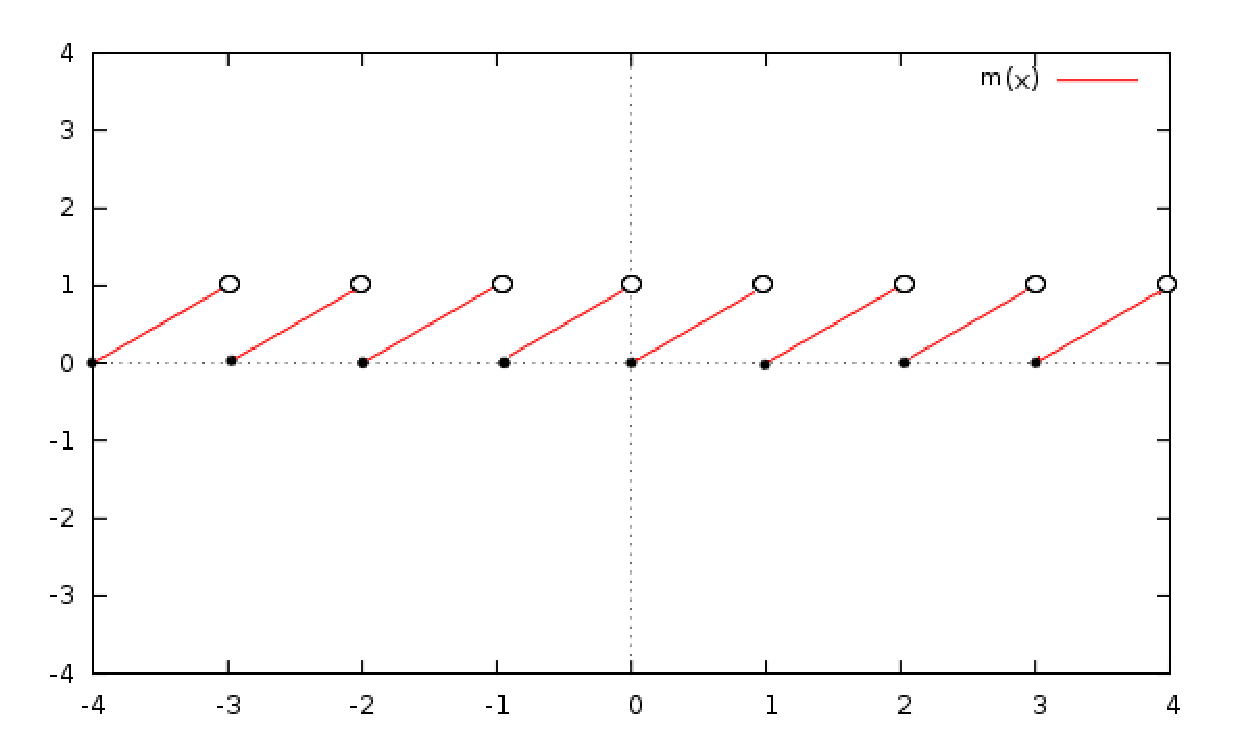
\includegraphics[height=4cm,width=6cm]{fmatis.eps} 
Dom$f = \mathbb{R}$, Cod$f = \mathbb{R}$, Im$f = [0,1)$\\
\end{center}
\end{minipage}
\hfill

\section{Paridad de Funciones Reales}
\subsection{Definición conjunto simétrico}
	Sea $D \subseteq \mathbb{R}$, diremos que es un conjunto simétrico sii: $x \in D \Rightarrow -x \in D$\\
	Ejemplo: $[-1,1]$ es simétrico pues: 
	$x \in [-1,1] \Leftrightarrow -1 \leqslant x \leqslant 1 \Leftrightarrow 
	-1 \leqslant -x < 1 \Leftrightarrow -x \in [-1,1]$
\subsection{Definición Paridad}
Sea $D$ un conjunto simétrico(respecto del origen) y sea $f:D \longrightarrow \mathbb{R}$ diremos que:
\subsubsection{Función Par}
\begin{center}
$f$ es una función par si y solo si 
$f(x)=f(-x)$, $ \forall x \in D$
\end{center}
\subsubsection{Función Impar}
\begin{center}
$f$ es una función impar si y solo si 
$f(x)=-f(-x)$, $ \forall x \in D$\\$\therefore$ $f(-x)=-f(x)$ la función es impar.
\end{center}
Nota: si el dominio $D$ no es simétrico no se puede hablar de ningun tipo de paridad.
\subsection{Interpretación gráfica} 
La gráfica de una función par es simétrica respecto aleje $y$ y la de una función impar es simétrica respecto del origen de coordenadas.\\

\hfill
\begin{minipage}{.45\textwidth}
\begin{center}
Grafica de $f(x)=x^{2}$
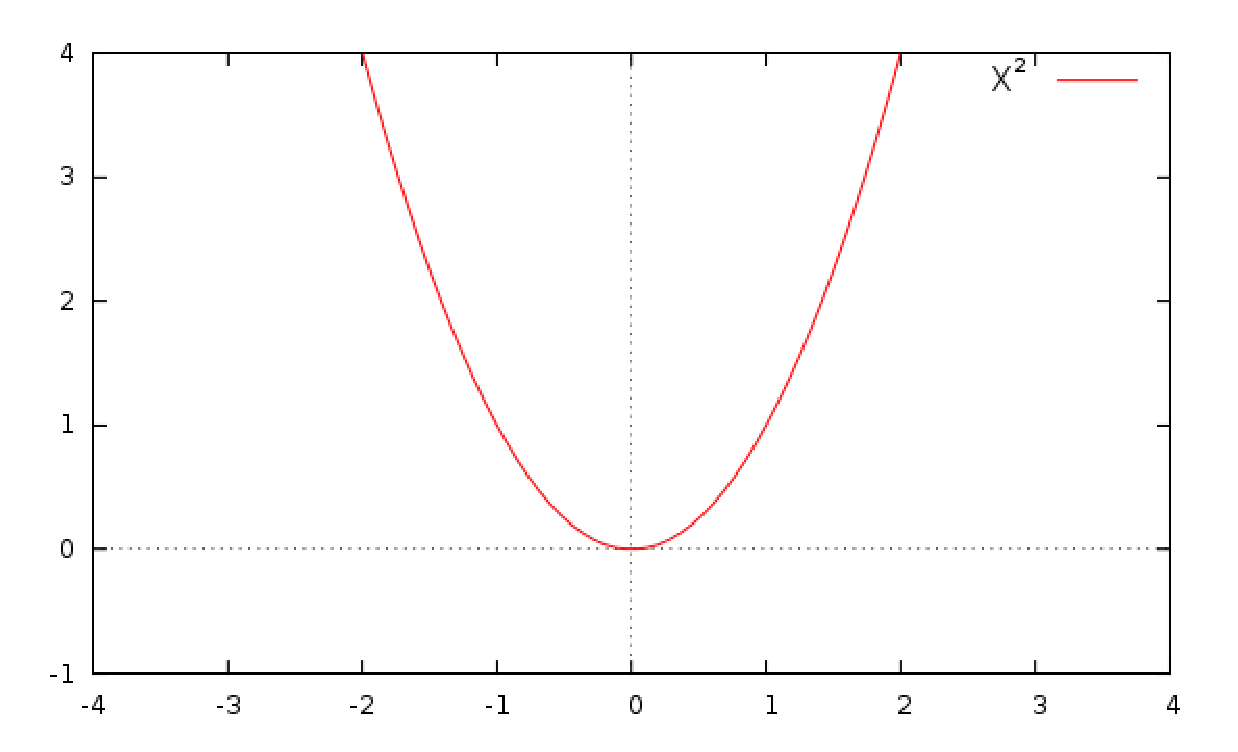
\includegraphics[height=4cm,width=6cm]{fxx.eps} 
Dom$f= \mathbb{R}$\\
$x^{2}$ es par ya que: $f(-x)=(-x)^{2}=x^{2}=f(x)$ 
\end{center}
\end{minipage}
\hfill
\begin{minipage}{.45\textwidth}
\begin{center}
Grafica de $f(x)=x^{3}$
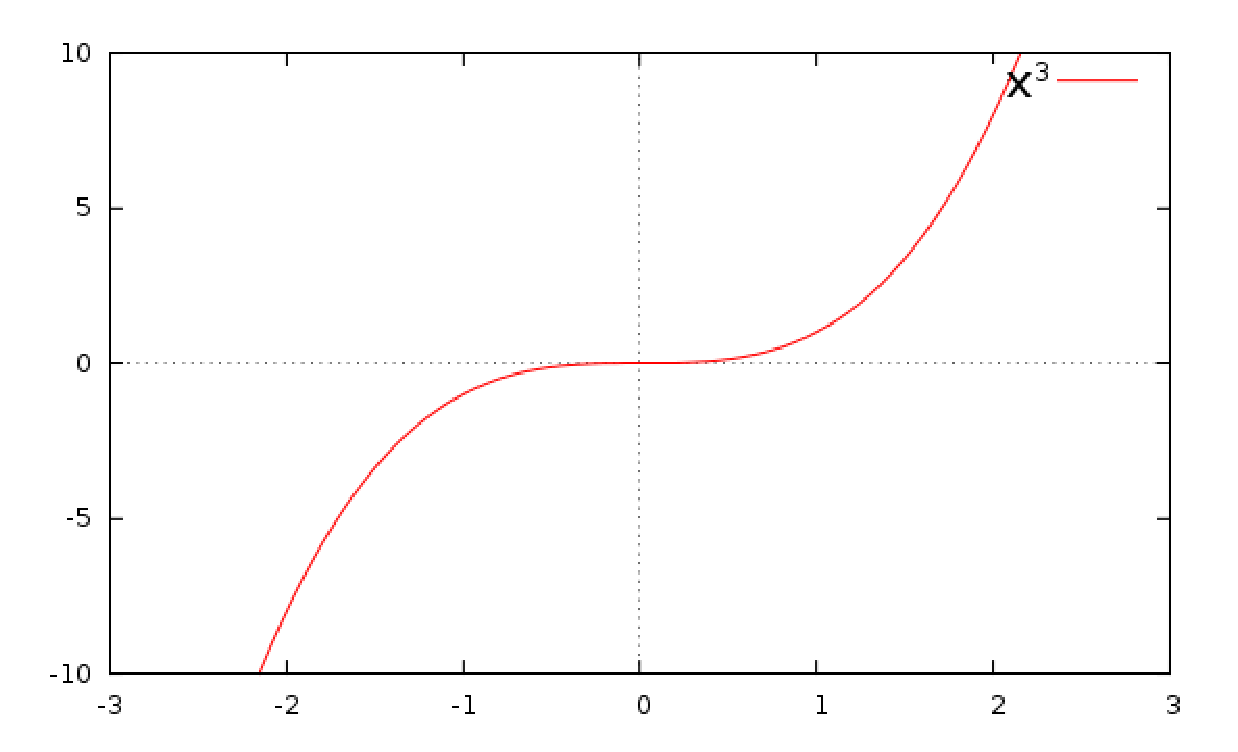
\includegraphics[height=4cm,width=6cm]{fxxx.eps} 
Dom$f= \mathbb{R}$ \\
$x^{3}$ es impar ya que: $f(-x)=(-x)^{3}=-x^{3}=-f(x)$ 
\end{center}
\end{minipage}
\hfill
\\\\

El conjunto de los $\mathbb{R}$ es simétrico.
\subsubsection{Ejemplo: $f(x)=x^{3}+x$}
\hfill
\begin{minipage}{.45\textwidth}
$f(x)=x^{3}+x$\\Dom$f=\mathbb{R}$ (simétrico)

Sea $x \in $ Dom$f$ , valido $f$ en $(-x)$
\begin{center}
$f(-x) = (-x)^{3}+(-x)=-(x^{3}+x)=-f(x) $\\ $\therefore$ la función es impar.
\end{center}
\end{minipage}
\hfill
\begin{minipage}{.45\textwidth}
\begin{center}
Grafica de $f(x)=x^{3}+x$
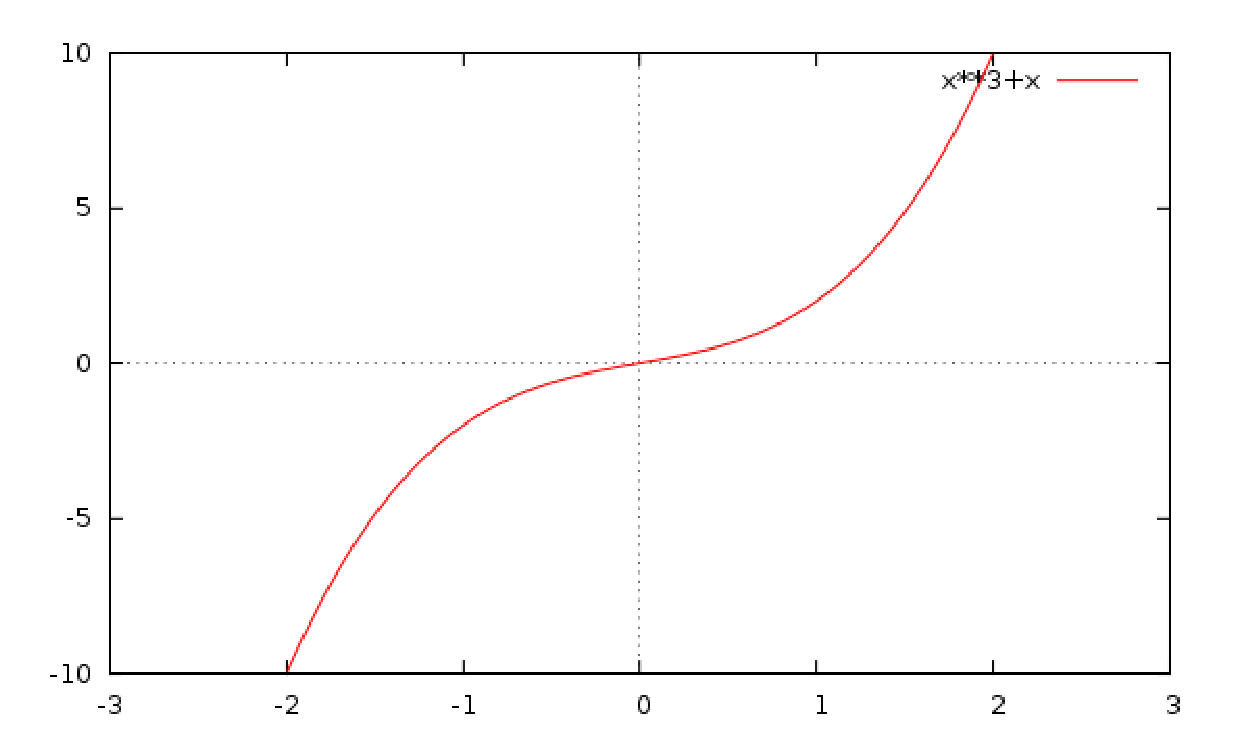
\includegraphics[height=4cm,width=6cm]{fxxx+x.eps} 
\end{center}
\end{minipage}
\hfill

\subsection{Propiedad de $f$ impar}
Sea $f$ una función impar y $0 \in $ Dom$f \Rightarrow f(0)=0$
\subsubsection{Demostración}
\begin{center}
$f(0)=-f(-0)\Rightarrow f(0)=-f(0) \Rightarrow$ \\
$\Rightarrow f(0)+f(0)=0 \Rightarrow 2 $ x $f(0)=0 \Rightarrow $\\
$\Rightarrow f(0)=\dfrac{0}{2} \Rightarrow f(0)=0$
\end{center} 
\subsection{Propiedad $f$ impar y par}
Sea $f$ una función par e impar a la vez, $f$ termina siendo la función nula, $f(x)=0$.
\subsubsection{Demostración}
\begin{center}

$f(x)\stackrel{f impar}{=}-f(-x)\stackrel{f par}{\Rightarrow}$
$f(x)=-f(x)$\\

$f(x)+f(-x)= 0 \Rightarrow$
$2$ x $f(-x)= 0$\\
$f(-x)= 0$
\end{center}
\section{Monotonía}

Definicion: Sea $f: D \longrightarrow \mathbb{R}$ diremos que:
\subsection{Funcion creciente}
$f$ es creciente en $D \Longleftrightarrow \forall x_{1}, x_{2} \in D / x_{1} < x_{2} \Rightarrow f(x_{1}) \leqslant f(x_{2})$
\subsection{Funcion estrictamente creciente}
$f$ es creciente en $D \Longleftrightarrow \forall x_{1}, x_{2} \in D / x_{1} < x_{2} \Rightarrow f(x_{1}) < f(x_{2})$
\subsection{Funcion decreciente}
$f$ es creciente en $D \Longleftrightarrow \forall x_{1}, x_{2} \in D / x_{1} < x_{2} \Rightarrow f(x_{1}) \geqslant f(x_{2})$
\subsection{Función estrictamente decreciente}
$f$ es creciente en $D \Longleftrightarrow \forall x_{1}, x_{2} \in D / x_{1} < x_{2} \Rightarrow f(x_{1}) > f(x_{2})$\\

Nota: Si bien $f$ es creciente o bien si es decreciente en todo su dominio, $f$ se dice monótona.
\subsection{Suma de funciones monótonas}
• La suma de dos funciones crecientes, es una función creciente.\\

• La suma de dos funciones decrecientes, es una función decreciente.
\subsubsection{Demostración  suma de funciones crecientes}
Hipotesis: $f:A\longrightarrow \mathbb{R}$,	$g:B\longrightarrow \mathbb{R}$	(ambas crecientes)\\

Definimos la función suma $f+g: A\cap B \longrightarrow \mathbb{R} /(f+g)_{(x)}=f(x)+g(x) $\\

Sean  $x_{1} < x_{2}; x_{1}, x_{2} \in A\cap B$

$x_{1}<x_{2} \stackrel{Hip}{\Rightarrow} \left\{
\begin{array}{c l}
f(x_{1})<f(x_{2})\\
f(g_{1})<g(x_{2})
\end{array}
\right. \Rightarrow 
f(x_{1})+g(x_{1}) \leqslant f(x_{2})+g(x_{2}) \Rightarrow
(f+g)_{(x_{1})} \leqslant (f+g)_{(x_{2})}$\\

$\therefore f+g$ es una función creciente.

\subsubsection{Demostración suma de funciones decrecientes}
Hipótesis: $f:A\longrightarrow \mathbb{R}$,	$g:B\longrightarrow \mathbb{R}$	(ambas decrecientes)\\

Definimos la función suma $f+g: A\cap B \longrightarrow \mathbb{R} /(f+g)_{(x)}=f(x)+g(x) $\\

Sean  $x_{1} < x_{2}; x_{1}, x_{2} \in A\cap B$

$x_{1}<x_{2} \stackrel{Hip}{\Rightarrow} \left\{
\begin{array}{c l}
f(x_{1})>f(x_{2})\\
f(g_{1})>g(x_{2})
\end{array}
\right. \Rightarrow 
f(x_{1})+g(x_{1}) \geqslant f(x_{2})+g(x_{2}) \Rightarrow
(f+g)_{(x_{1})} \geqslant (f+g)_{(x_{2})}$\\

$\therefore f+g$ es una función decreciente.

\section{Función Lineal}
\hfill
\begin{minipage}{.45\textwidth}
$$g: \mathbb{R} \longrightarrow \mathbb{R} / g(x)= m x + h$$
\end{minipage}
\hfill
\begin{minipage}{.45\textwidth}
$m$ : Pendiente.\\
$x$ : Variable independiente.\\
$h$ : Ordenada al origen.\\
\end{minipage}
\hfill
\subsection{Casos de funciones lineales}
\subsubsection{Caso $m=0$}
\begin{center}
$m=0 \Rightarrow g(x)=h$\\$ \therefore g(x)$ es constante.
\end{center}
\subsubsection{Caso $m>0$}
\hfill
\begin{minipage}{.45\textwidth}
$m>0 \Rightarrow g(x)= mx+h$\\

Sean  $x_{1} < x_{2}; x_{1}, x_{2} \in \mathbb{R}$
\begin{center}
$x_{1} < x_{2} \stackrel{m > 0}{\Rightarrow} mx_{1}  < mx_{2} \Rightarrow$\\
 $mx_{1}+h < mx_{2}+h \Rightarrow g(x_{1}) < g(x_{2})$\\
 $\therefore$ es una función estrictamente creciente  
\end{center}
\end{minipage}
\hfill
\begin{minipage}{.45\textwidth}
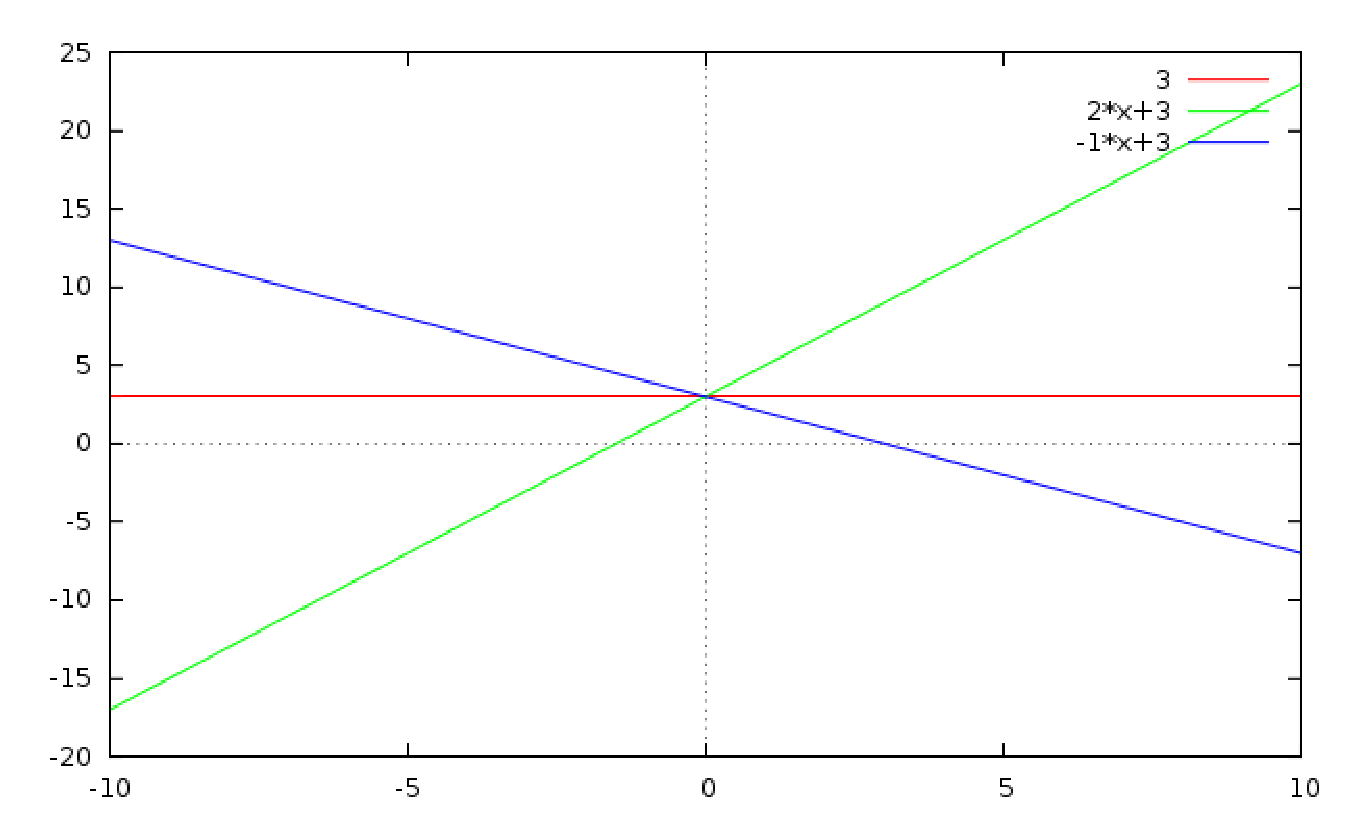
\includegraphics[height=4cm,width=6cm]{flinealcasos.eps} 
\begin{center}
$f(x)=mx+3$ con $m=-1< 0$ y $m=1>0$
\end{center} 
\end{minipage}
\hfill
\subsubsection{Caso $m<0$}
$m<0 \Rightarrow g(x)= mx+h$\\

Sean  $x_{1} < x_{2}; x_{1}, x_{2} \in \mathbb{R}$
\begin{center}
$x_{1} < x_{2} \stackrel{m < 0}{\Rightarrow} mx_{1}  > mx_{2} \Rightarrow$\\
 $mx_{1}+h > mx_{2}+h \Rightarrow g(x_{1}) > g(x_{2})$\\
 $\therefore$ es una función estrictamente decreciente  
\end{center}

\subsection{Pendiente}
La pendiente es la inclinación de la recta. Suponiendo que nuestra pendiente es $\alpha$, sera $tg(\alpha)= m$. Siendo este $m$ el mismo que e de nuestra ecuación $mx+h$.
\subsection{Intersección con el eje $Y$}
$$x=0 \Rightarrow y=f(0) \Rightarrow y=m.0+h \Rightarrow y=h$$
\subsection{Interseccion con el eje $X$}
$$y=0 \Rightarrow 0=f(x) \Rightarrow 0=mx+h \Rightarrow x=\dfrac{-h}{m}$$
\section{Periodicidad}
Si existe una constante positiva $p / \forall x \in D, x+p \in D$ y $f(x+p)=f(x)$. $f$ se dice periódica y al mínimo $p$ que verifica $f(x+p)=f(x)$ se o llama periodo de la función $f$.
\subsection{Ejemplo: función Mantisa}
$f: \mathbb{R} \longrightarrow \mathbb{R}/f(x)= x-\lfloor x \rfloor$\\

Primero veamos que sucede si $p \in \mathbb{Z}, \Rightarrow \lfloor x+p \rfloor = \lfloor x \rfloor +p$
$$f(x+p) = (x+p)-(\lfloor x+p \rfloor) \underset{p \in \mathbb{Z}}{\Rightarrow} f(x+p) = x+p-\lfloor x \rfloor - p
\Rightarrow f(x+p) = x-\lfloor x \rfloor = f(x)$$

Esto se cumple para todo $p \in \mathbb{Z}$.\\

Vimos que con un numero perteneciente a $\mathbb{Z}$ se cumple parte de la condición de periodicidad pero, esta también dice que el periodo es el mínimo. Por lo tanto buscamos el mínimo de los naturales positivo y hallamos el numero $1$.\\

Conclusión el periodo de la función Mantisa es $1$.
\section{Traslaciones}
Movimientos de las representaciones gráficas.\\
Sea $f:D \longrightarrow \mathbb{R} / x\longrightarrow y=f(x)$ :
\subsection{Traslación Vertical}
\hfill
\begin{minipage}{.45\textwidth}
Sea $g(x)= f(x)+c$ con $c \in \mathbb{R}$\\

• Si $c>0$ la gráfica de $g$ se obtiene desplazando la de $f$ una distancia $|c|$ asia arriba.\\

• Si $c<0$ la gráfica de $g$ se obtiene desplazando la de $f$ una distancia $|c|$ asia abajo. 
\end{minipage}
\hfill
\begin{minipage}{.45\textwidth}
\begin{center}
Ejemplo $f(x)=|x|$
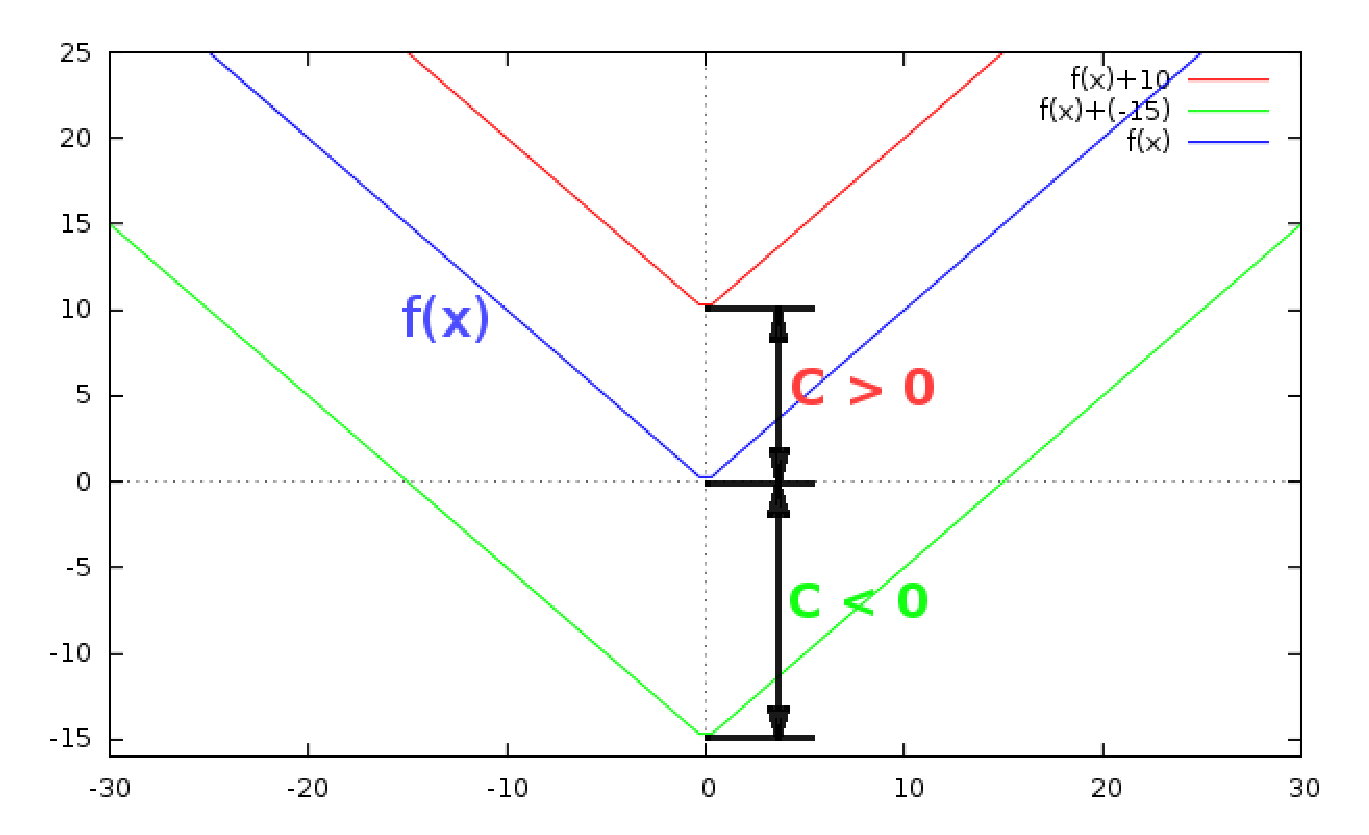
\includegraphics[height=4cm,width=6cm]{transV.eps} 
\end{center} 
\end{minipage}
\hfill

\subsection{Traslación Horizontal}
\hfill
\begin{minipage}{.45\textwidth}
Sea $g(x)= f(x-c)$ con $c \in \mathbb{R}$\\
Dom$f=$\{$x \in \mathbb{R} /x-c \in $Dom$f$\}\\

• Si $c>0$ la gráfica de $g$ se obtiene desplazando la de $f$ una distancia $|c|$ asia la derecha.\\

• Si $c<0$ la gráfica de $g$ se obtiene desplazando la de $f$ una distancia $|c|$ asia la izquierda. 
\end{minipage}
\hfill
\begin{minipage}{.45\textwidth}
\begin{center}
Ejemplo $f(x)=|x|$
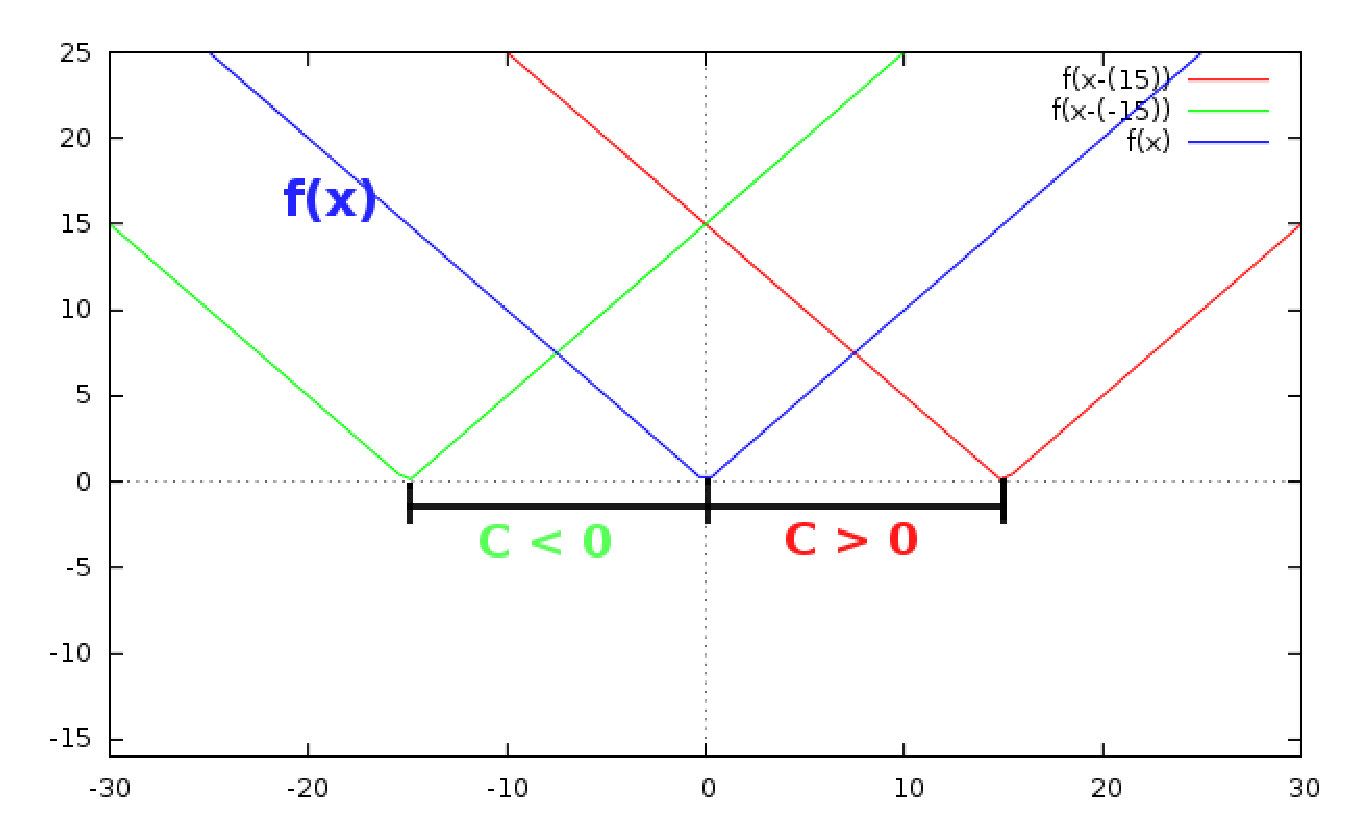
\includegraphics[height=4cm,width=6cm]{transH.eps} 
\end{center} 
\end{minipage}
\hfill
\newpage
\section{Dilataciones y contracciones}
Sea $c >0$:
\subsection{Dilataciones y contracciones verticales}
\hfill
\begin{minipage}{.45\textwidth}

• $y=cf(x)$ dilata o estira la gráfica de $f$ verticalmente de por un factor $c$.

• $y=\dfrac{1}{c}f(x)$ comprime la gráfica de $f$ verticalmente de por un factor $c$.
 
\end{minipage}
\hfill
\begin{minipage}{.45\textwidth}
\begin{center}
Ejemplo $f(x)=sen(x)$ en roja, $c=2$. Verde dilatación, azul contracción. 
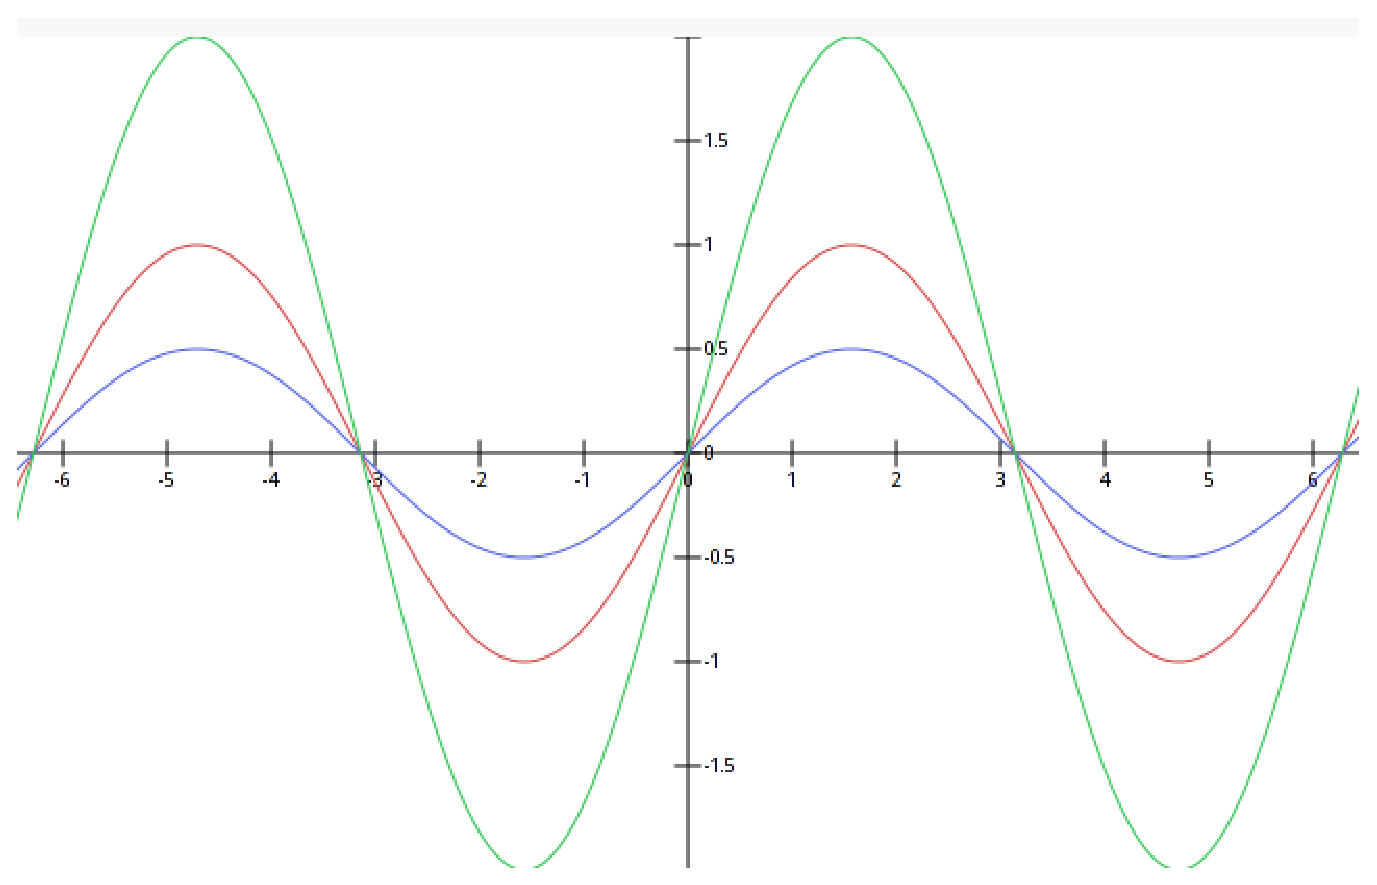
\includegraphics[height=4cm,width=6cm]{dicover.eps} 
\end{center} 
\end{minipage}
\hfill


\subsection{Dilataciones y contracciones horizontales}



\hfill
\begin{minipage}{.45\textwidth}

• $y=f(xc)$ dilata o estira la gráfica de $f$ horizontalmente por un factor $c$.

• $y=f(x \dfrac{1}{c})$ comprime la gráfica de $f$ horizontalmente por un factor $c$.
 
\end{minipage}
\hfill
\begin{minipage}{.45\textwidth}
\begin{center}
Ejemplo $f(x)=sen(x)$ en roja, $c=2$. Verde dilatación, azul contracción. 
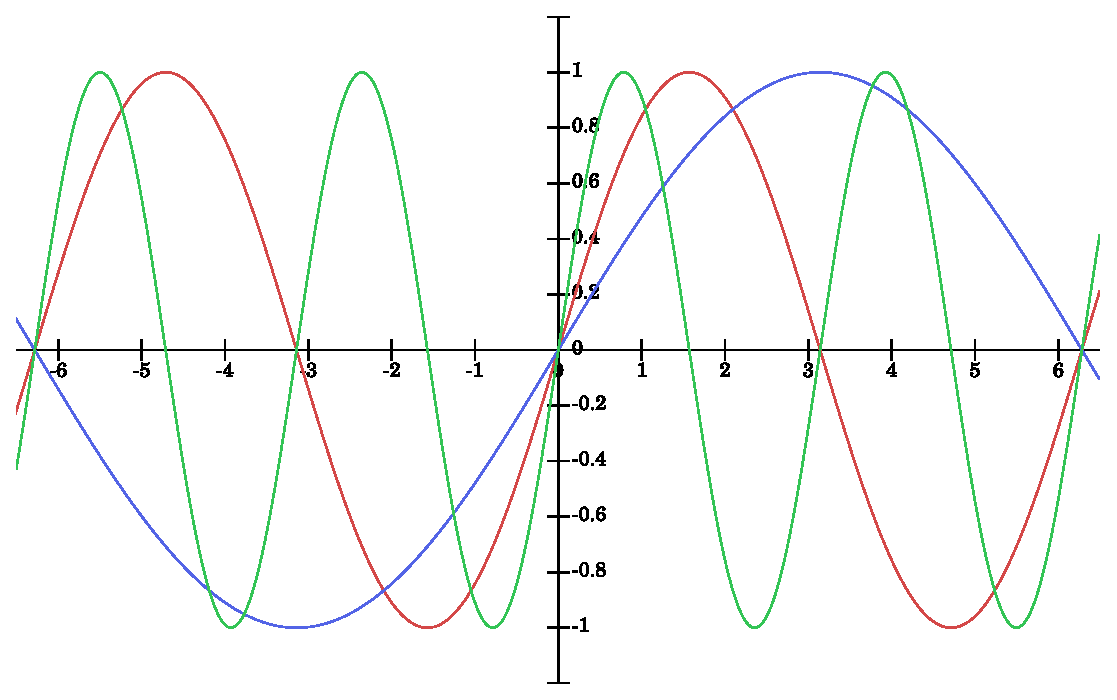
\includegraphics[height=4cm,width=6cm]{dicoho.eps} 
\end{center} 
\end{minipage}
\hfill

\section{Reflexiones respecto a los ejes}
\subsection{Reflexión en el eje $X$}
\hfill
\begin{minipage}{.45\textwidth}
Sea $f: D \longrightarrow \mathbb{R}/ y=f(x)$\\
defiimos $g(x)= (-1) f(x)$, Dom$f=$Dom$f$\\
Si $(x, y) \in $ Gr$(f) \Rightarrow (x, -y) \in $ Gr$(g)$\\

Nota: Si $w$ es raíz de $f$, es decir $f(w)=0$, entonces $w$ también lo es de $g$.
\end{minipage}
\hfill
\begin{minipage}{.45\textwidth}
\begin{center}
Ejemplo $f(x)=|x|$ , en roja. La reflexión esta en azul. 
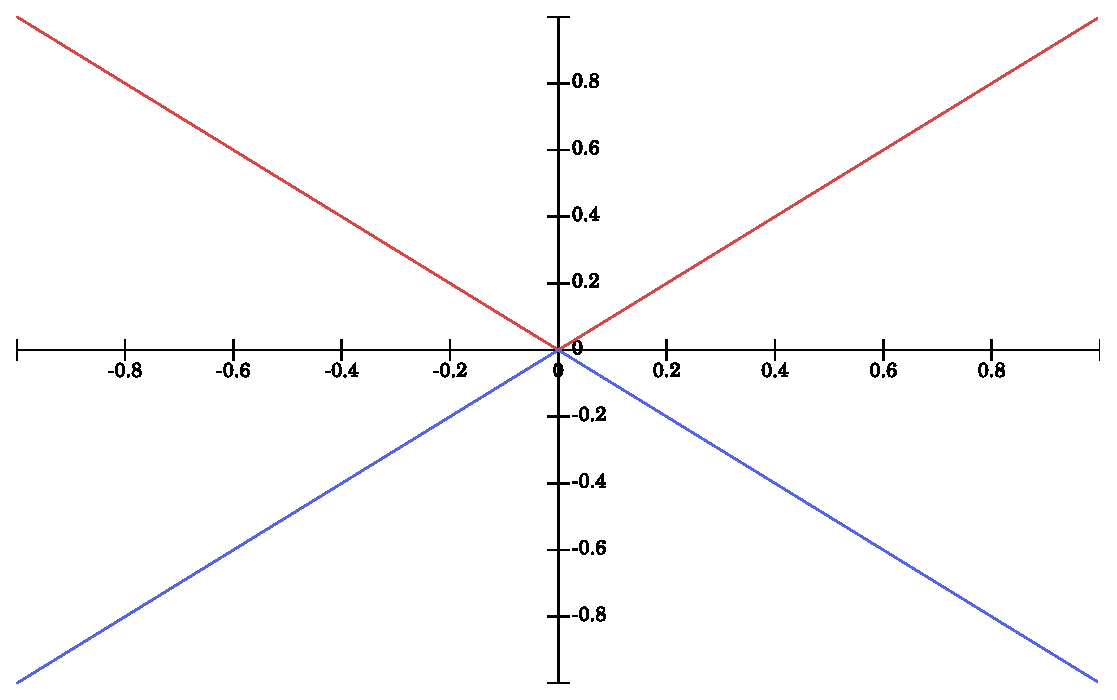
\includegraphics[height=4cm,width=6cm]{refx.eps} 
\end{center} 
\end{minipage}
\hfill
\subsection{Reflexión en el eje $Y$}
\hfill
\begin{minipage}{.45\textwidth}
Sea $f: D \longrightarrow \mathbb{R}/ y=f(x)$\\
defiimos $g(x)=  f(x(-1))$\\
Dom$f=$\{$x \in \mathbb{R} / -x \in $ Dom$f$\} \\
Si $(x, y) \in $ Gr$(f) \Rightarrow (-x, y) \in $ Gr$(g)$\\

Nota: se conserva la ordenada al origen y no cambia la imagen.
\end{minipage}
\hfill
\begin{minipage}{.45\textwidth}
\begin{center}
Ejemplo $f(x)=x$ , en roja. La reflexión esta en azul. 
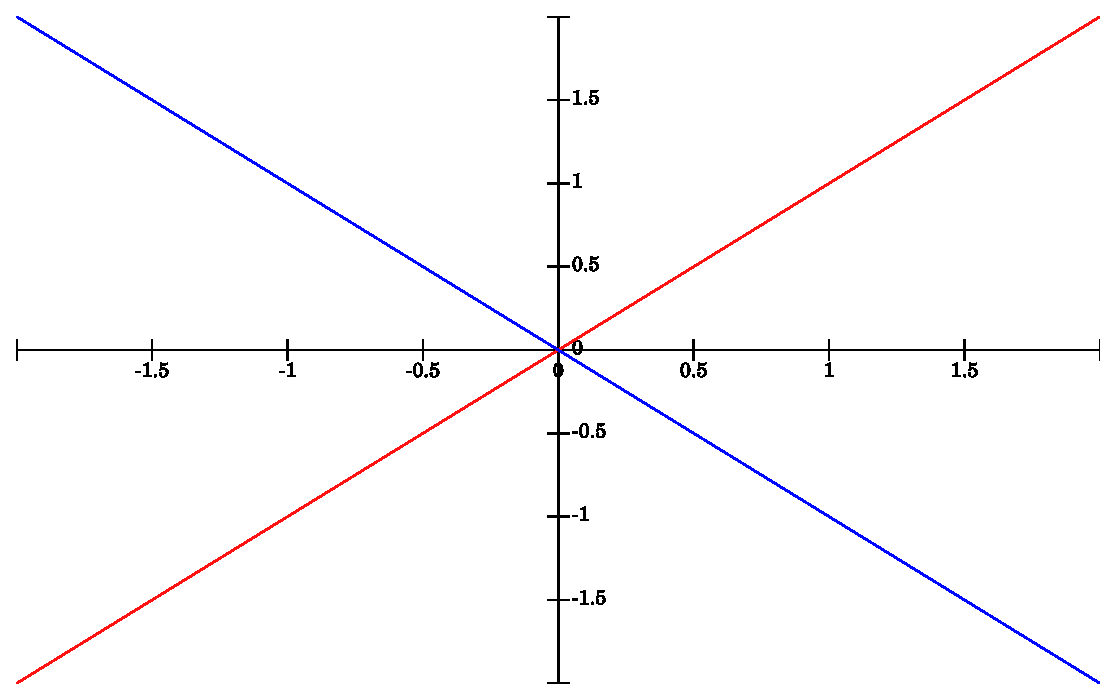
\includegraphics[height=4cm,width=6cm]{refy.eps} 
\end{center} 
\end{minipage}
\hfill
\section{Valor absoluto de una función}
\hfill
\begin{minipage}{.45\textwidth}
Sea $f:D \longrightarrow \mathbb{R} / y= f(x)$\\
definimos $g(x)=|f(x)|$\\
es decir:\\
$g(x)=\left\{
\begin{array}{c l}
  f(x) & f(x)>0 \\
  -f(x) & f(x)<0
\end{array}
\right.$\\
Dom$f=$Dom$g$

\end{minipage}
\hfill
\begin{minipage}{.45\textwidth}
\begin{center}
Ejemplo $f(x)=|sin(x)|$
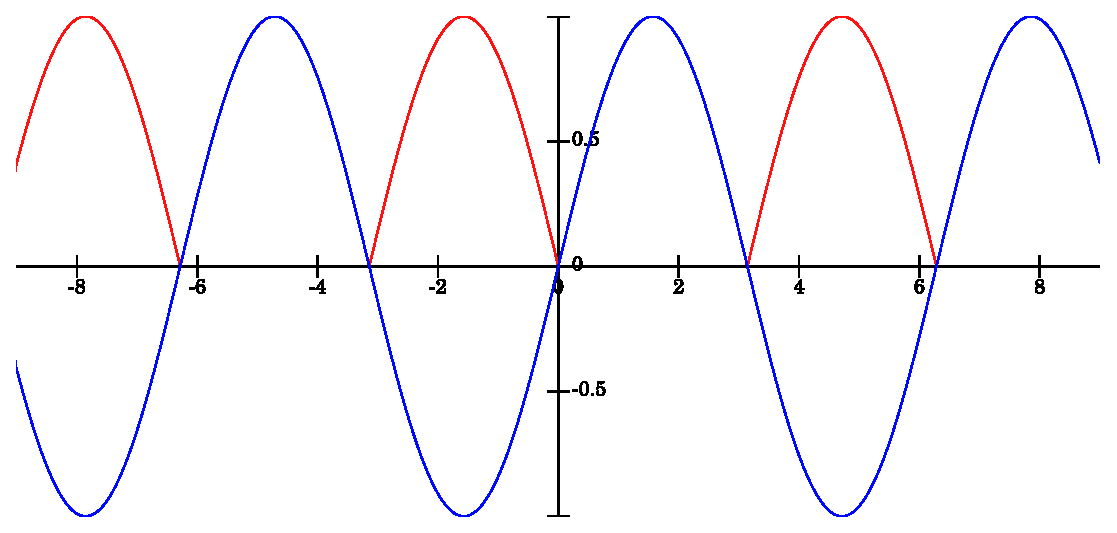
\includegraphics[height=4cm,width=6cm]{abssinx.eps} 
\end{center} 
\end{minipage}
\hfill
\section{Función Cuadrática}
\subsection{Función cuadrática elemental}
\hfill
\begin{minipage}{.45\textwidth}
Estudiaremos primero la función elemental:\\
\begin{center}
$f:\mathbb{R} \longrightarrow \mathbb{R}$

$x \longrightarrow f(x)=x^{2}$
\end{center}
Dom$f = \mathbb{R}$\\
Cod$f = \mathbb{R}$\\
Im$f = \mathbb{R} ^{+} _{0}$\\
\end{minipage}
\hfill
\begin{minipage}{.45\textwidth}
\begin{center}
Función cuadrática elemental
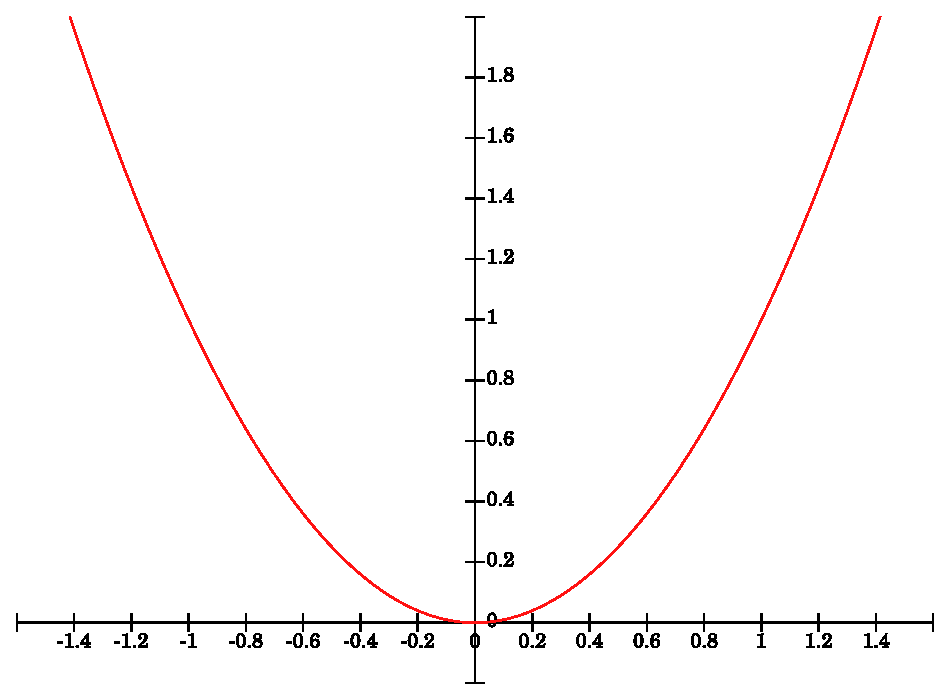
\includegraphics[height=4cm,width=6cm]{fcxx.eps} 
\end{center} 
\end{minipage}
\hfill

• GR$(f)=$\{$(x,y) \in \mathbb{R}^{2} / y= x^{2}$\} $=$ \{$(x,x^{2}); x \in \mathbb{R}$\}

• Es par pues: $f(-x)=(-x)^{2}=f(x)$, $\forall x \in \mathbb{R}$

• $f$ es creciente estrictamente en $(0,+\infty)$

Sean $x_{1},x_{2} \in (0,+\infty)$ y $x_{1} < x_{2}$\\

$$x_{1} < x_{2} \underset{\stackrel{x_{1}>0}{\stackrel{x_{2}>0}{}}}{\Rightarrow}x_{1}^{2}<x_{2}^{2} \Rightarrow f(x_{1})<f(x_{2})$$

• $f$ es estrictamente decreciente en $(-\infty,0)$, ya que es par y estrictamente creciente en $(0,+\infty)$.

\subsection{Definición de función cuadrática}
 Una ``Función Cuadrática'' es una función definida por:
 \begin{center}
 $f: \mathbb{R} \longrightarrow \mathbb{R} / f(x)= ax^{2}+bx+c$, Donde $a,b,c \in \mathbb{R}$ y $a \neq 0$ 
 \end{center}

\subsection{Gráfica de la función cuadrática}  

Como ya conocemos la gráfica de la función cuadrática elemental $(f(x)=x^{2})$, la idea es transformar nuestra función cuadrática en corrimientos de la función cuadrática elemental y así poder hallar su gráfica mucho mas fácil.

Tenemos $f(x)=ax^{2}+bx+c$
\begin{center}
$$a.x^{2}+b.x+c $$\\
= $\langle$ factor común $a \rangle$\\
$$a \left[ x^{2}+\dfrac{b}{a}x+\dfrac{c}{a}\right]$$\\
= $\langle$ multiplicoy divido $\left(\dfrac{b}{a}x\right)$ por $2 \rangle$\\
$$a\left[ x^{2}+2\dfrac{b}{2a}x+\dfrac{c}{a}\right]$$\\
= $\langle$ sumo  y resto $\left(\dfrac{b}{a}x\right)^{2}$ para completar cuadrado $\rangle$\\
$$a \left[ x^{2}+2\dfrac{b}{2a}x+\left(\dfrac{b}{a}x\right)^{2}-\left(\dfrac{b}{a}x\right)^{2}+\dfrac{c}{a}\right]$$\\
= $\langle$ aplico inversa del trinomio cuadrado perfecto $\rangle$\\
$$a \left[ \left(x+\dfrac{b}{2a}\right)^{2}-\left( \dfrac{b}{2a}\right)^{2}+\dfrac{c}{a}\right]$$\\
= $\langle$ propiedad de potencia y resuelvo $\rangle$\\
$$a \left[ \left(x+\dfrac{b}{2a}\right)^{2}- \dfrac{b^{2}}{4a^{2}}+\dfrac{c}{a}\right]$$\\
= $\langle$ resuelvo la suma de fracciones $:\left\{
\begin{array}{c l}
  \dfrac{-b^{2}}{4a^{2}}+\dfrac{c}{a} \\
  $denominador común$\\
  \dfrac{-b^{2}+c4a}{4a^{2}}
\end{array}
\right.\rangle$\\

$$a\left[ \left( x+ \dfrac{b}{2a} \right) ^{2} + \dfrac{-b^{2}+c4a}{4a2}\right]$$\\
= $\langle$ distribuyo $a\rangle$\\
$$a\left(x+\dfrac{b}{2a}\right)^{2}+\frac{-b^{2}+c4a}{4a}$$\\
= $\langle$ si llamamos a $p=\dfrac{-b}{2a}$, y a $q=\dfrac{-b^{2}+4ac}{4a} $, resulta $\rangle$\\
$$a(x-p)^{2}+q$$
\end{center}

\subsubsection{Raíces de la función cuadrática (intersección con el eje $X$)}

$$f(x)=0 \Leftrightarrow a\left(x+\dfrac{a}{2a}\right)^{2}+\dfrac{-b^{2}+4ac}{4a}=0 \Leftrightarrow
a\left(x+\dfrac{a}{2a}\right)^{2}=-\dfrac{-b^{2}+4ac}{4a} \Leftrightarrow $$ $$
 \left(x+\dfrac{a}{2a}\right)^{2}=\dfrac{b^{2}-4ac}{4a^{2}} \Leftrightarrow x+\dfrac{b}{2a}=\pm\sqrt{\dfrac{b^{2}-4ac}{4a^{2}}} \Leftrightarrow $$ $$
 \Leftrightarrow x =\dfrac{-b}{2a}\pm\dfrac{\sqrt{b^{2}-4ac}}{2a}\Leftrightarrow  x=\dfrac{-b\pm\sqrt{b^{2}-4ac}}{2a}$$
 
$$ \therefore f(x)=0 \Rightarrow x_{1,2}=\left. \dfrac{-b\pm\sqrt{b^{2}-4ac}}{2a}\right\} resolvente$$
\subsubsection{Discriminante de la resolvente ``$\bigtriangleup$''}

Llamamos discriminante de la resolvente a el numero real:
$$\bigtriangleup = b^2 -4ac$$

Hora veremos porque es importante el discriminante, es que al ver los posibles valores q puede tomar la resolvente nos dará distinguibles resultados:

$$x_{1,2}= \dfrac{-b\pm\sqrt{ \bigtriangleup }}{2a}$$

\paragraph{Caso $\bigtriangleup = 0$}
\begin{center}
$f(x)=0 \Leftrightarrow x_{1,2}= \dfrac{-b\pm\sqrt{0}}{2a} 
\Leftrightarrow x_{1,2}= \dfrac{-b}{2a} $ \qquad (Raiz $\mathbb{R}$ doble)\\

La Gr$f$ corta al eje $X$ en un solo punto: $x=\dfrac{-b}{2a}$.
\end{center}

\paragraph{Caso  $\bigtriangleup > 0$}
\begin{center}
$f(x)=0 \Leftrightarrow x_1= \dfrac{-b + \sqrt{b^{2}-4ac}}{2a} 
$ \quad$ \bigwedge $ \quad$ x_2=\dfrac{-b-\sqrt{b^{2}-4ac}}{2a}
$ \qquad (2 raices $\mathbb{R}$ distintas)\\

La Gr$f$ corta al eje $X$ en dos puntos: $x_1$ y $x_2$.
\end{center}

\paragraph{Caso  $\bigtriangleup < 0$}
\begin{center}
$f(x)=0 \Leftrightarrow x_{1,2}=\dfrac{-b\pm\sqrt{b^{2}-4ac}}{2a}$ \qquad (Existen 2 raices $\mathbb{C}$ opuestas)\\

La Gr$f$ corta al eje $X$ en dos puntos: $x_1$ y $x_2$.
\end{center}
\subsubsection{Ejemplos de gráficas:}

• Considerece $a>0$
\\
\\
\hfill
\begin{minipage}{.20\textwidth}
$$\bigtriangleup<0$$
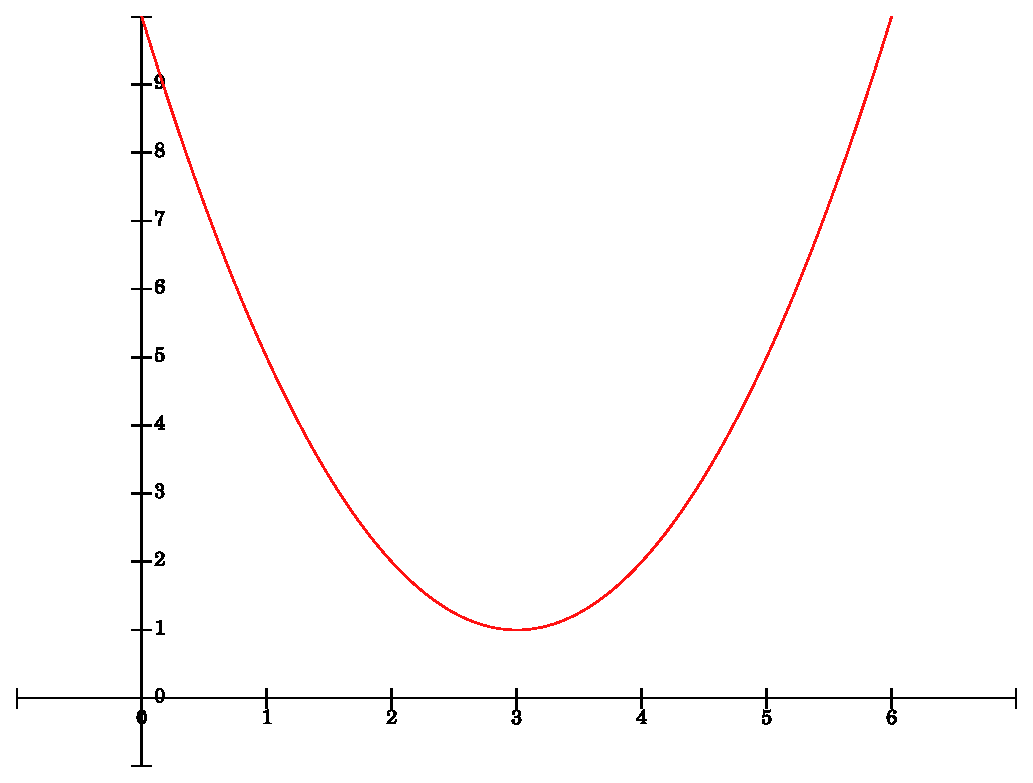
\includegraphics[height=4cm,width=4cm]{xx1.eps} 

\end{minipage}
\hfill
\begin{minipage}{.20\textwidth}
$$\bigtriangleup=0$$
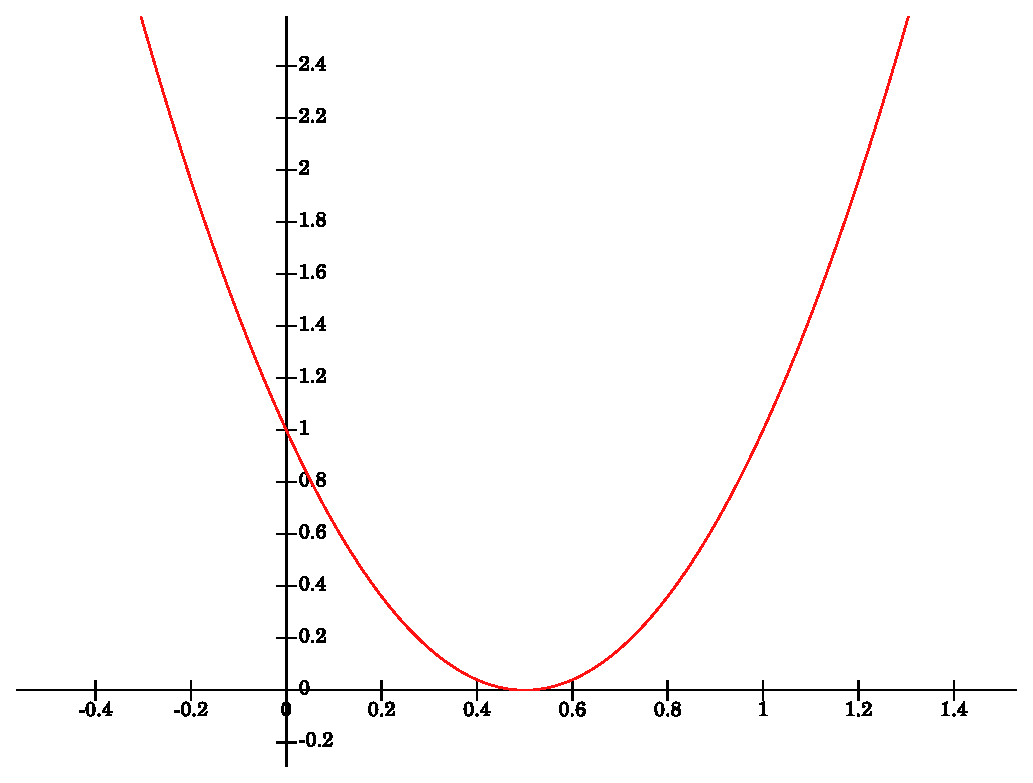
\includegraphics[height=4cm,width=4cm]{xx4.eps} 
\end{minipage}
\hfill
\begin{minipage}{.20\textwidth}
$$\bigtriangleup>0$$
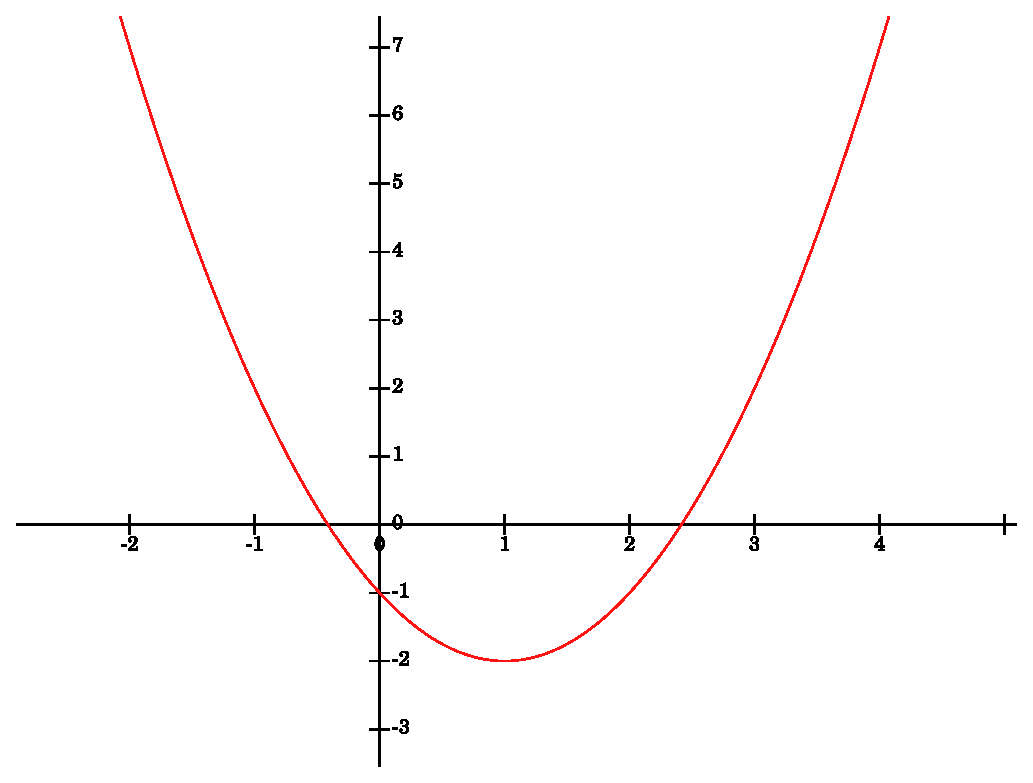
\includegraphics[height=4cm,width=4cm]{xx5.eps} 

\end{minipage}
\hfill
\\
\\

• Considérese $a<0$
\\
\\
\hfill
\begin{minipage}{.20\textwidth}
\begin{center}
$\bigtriangleup<0$
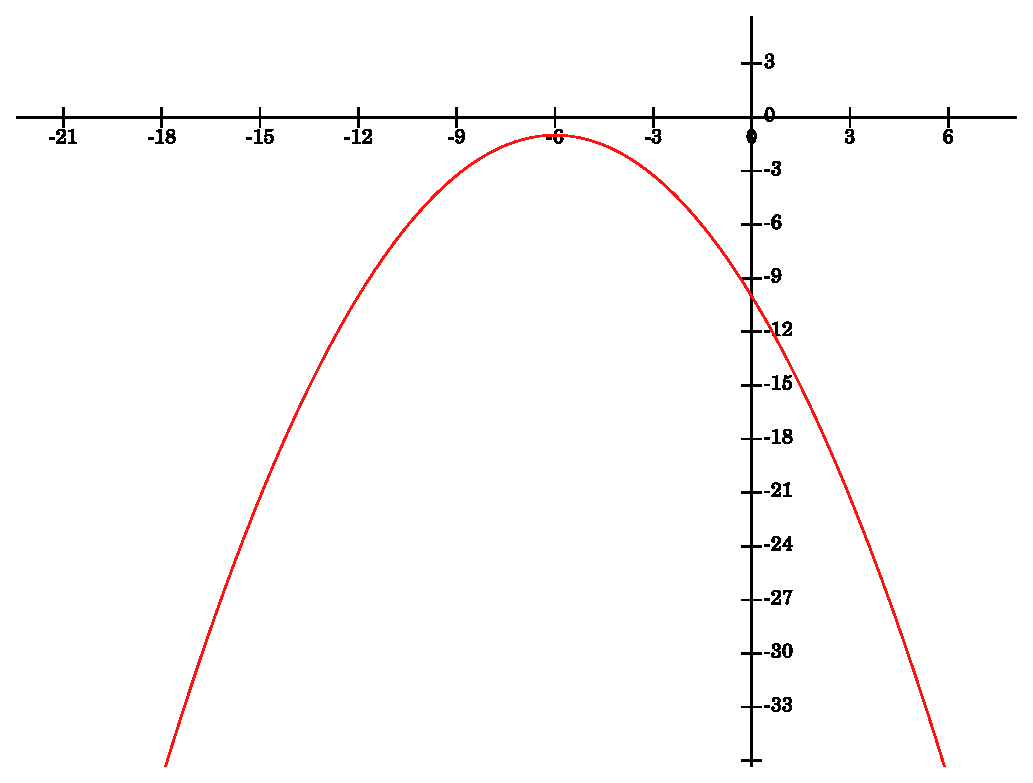
\includegraphics[height=4cm,width=4cm]{xx2.eps} 
\end{center} 
\end{minipage}
\hfill
\begin{minipage}{.20\textwidth}
\begin{center}
$\bigtriangleup=0$
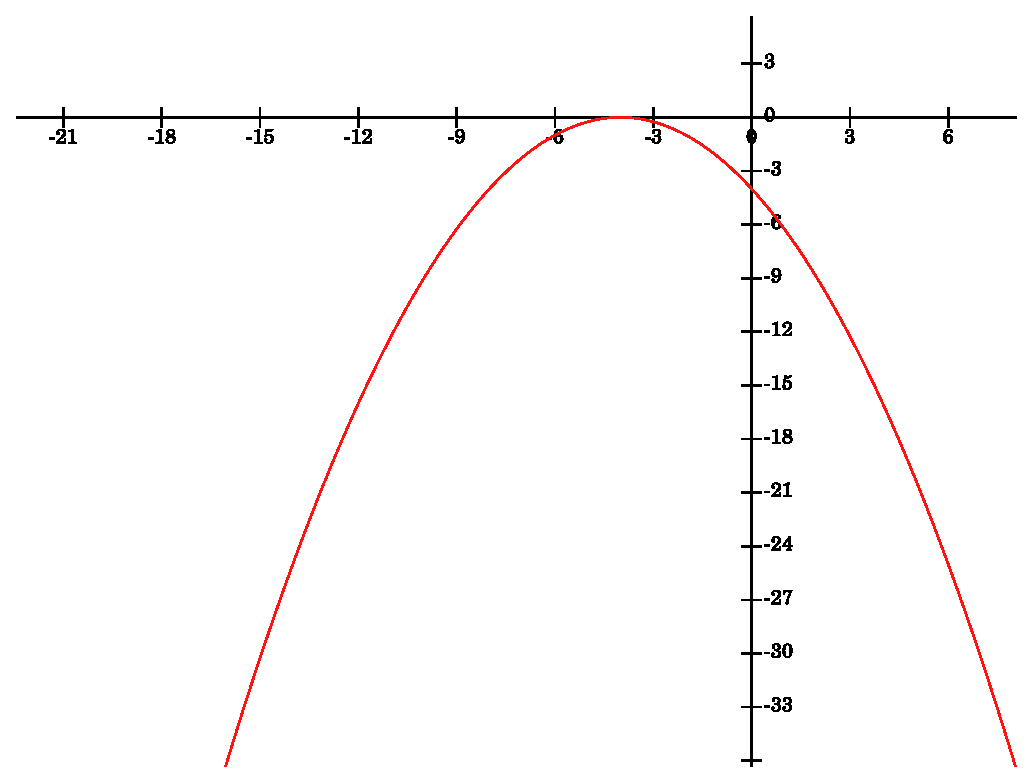
\includegraphics[height=4cm,width=4cm]{xx3.eps} 
\end{center} 
\end{minipage}
\hfill
\begin{minipage}{.20\textwidth}
\begin{center}
$\bigtriangleup>0$

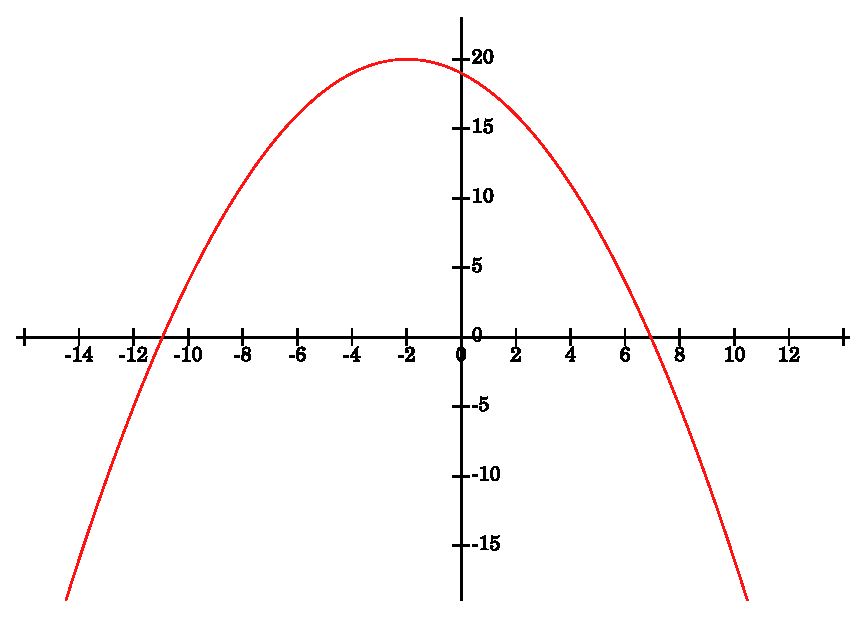
\includegraphics[height=4cm,width=4cm]{xx6.eps} 
\end{center} 
\end{minipage}
\hfill


\subsubsection{Intersección con el eje $Y$}

$$f(0)= a \times 0 + b \times 0 + c \Rightarrow f(0)= c$$

La Gr$f$ corta al eje y en el punto $(0, c)$
\subsubsection{Vertiese } 

El punto vértice en la gráfica de la función cuadrática se determina por 
los siguientes valores:

\paragraph{Eje de simetría}
\quad \\El eje de simetría de la función cuadrática es $x = p$ \\
por tanto: $ x = \dfrac{-b}{2a} $

\paragraph{Máximo o Mínimo de la funciona cuadrática}
 
\quad \\El máximo o mínimo de una función cuadrática en el eje $Y$ \\
 lo determina el valor de $q$ es decir: $\dfrac{-b^{2}+4ac}{4a}$\\\\\\
Por lo tanto el vértice queda conformado como $(p, q)$ es decir:
$$ V\left( \dfrac{-b}{2a} , \dfrac{-b^{2}+4ac}{4a}\right)$$
\newpage
\subsection{Ejemplo de una función cuadrática}

Dada:
$$ f : \mathbb{R} \longrightarrow \mathbb{R} / x \longrightarrow f(x) = 2x^2-5x+2$$\\
\hfill
\begin{minipage}{.45\textwidth}
\begin{center}
$2x^2-5x+2 $\\
$= \quad \langle$ factor común 2 $\rangle$\\
$ 2 \left[ x^2 - x \times \dfrac{5}{2}  +1 \right] $\\
$= \quad \langle$ multiplico y divido por 2 $\rangle$\\
$ 2 \left[ x^2 - x \times \dfrac{5\times 2}{2\times 2}  +1 \right] $\\
$= \quad \langle$ sumo y resto $\left(\dfrac{5}{4}\right)^2$ $\rangle$\\
$ 2 \left[ x^2 - 2 \times x \times \dfrac{5}{4} + \dfrac{25}{16} -\dfrac{25}{16}  +1 \right] $\\
$= \quad \langle$ trinomio cuadrado perfecto; resuelvo fracciones $\rangle$\\
$ 2 \left[ \left(x-\dfrac{5}{4} \right)^2 - \dfrac{9}{16} \right] $\\
$= \quad \langle$ distrivullo el 2  y simplifico $\rangle$\\
$ 2 \left(x-\dfrac{5}{4} \right)^2 - \dfrac{9}{8} $\\
\end{center}
\end{minipage}
\hfill
\begin{minipage}{.45\textwidth}
\begin{center}

Grafica de $f(x)$
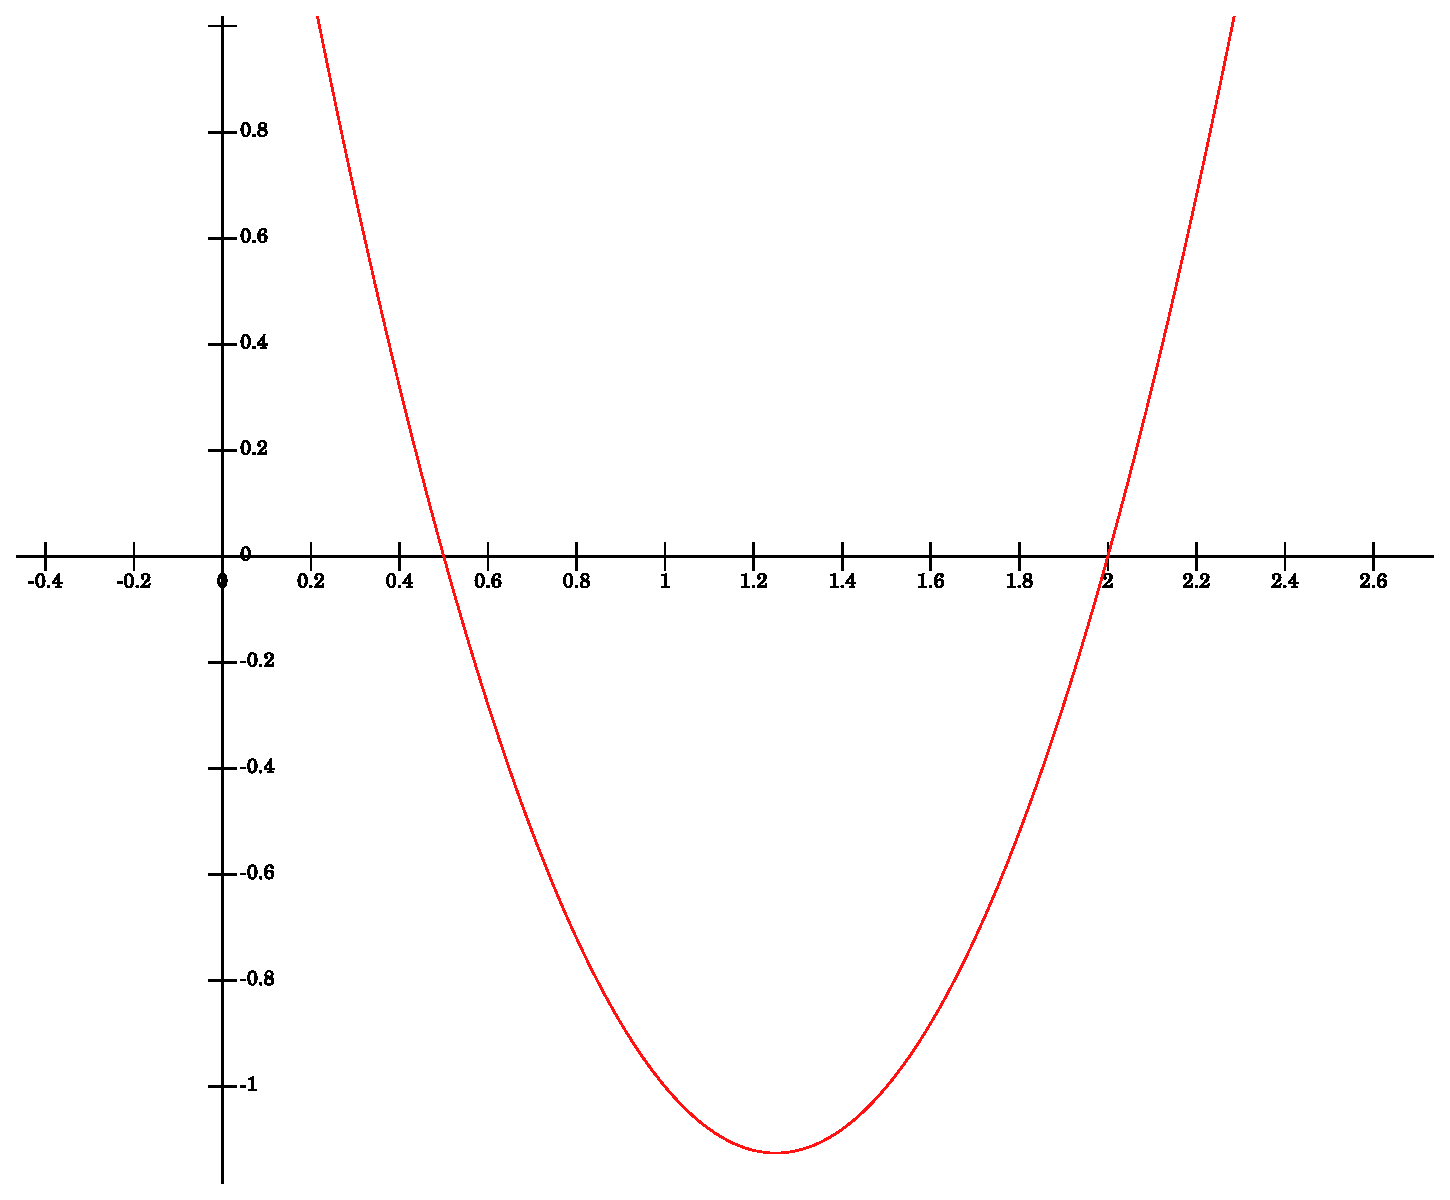
\includegraphics[height=8cm,width=8cm]{fejxx.eps} 
\end{center}
\end{minipage}
\hfill \\ \\

• Hallamos el vértice: $V\left(\dfrac{5}{4},-\dfrac{9}{8} \right)$


• Intersección con ele eje $Y$: $f(0)= 2\times 0^2-5\times 0+2 = 2 $


• Raíces:
\\

\hfill
\begin{minipage}{.45\textwidth}
$2 \times \left( x -\dfrac{5}{4}\right)^2 -\dfrac{9}{8} =0 \Leftrightarrow 
2 \times \left( x -\dfrac{5}{4}\right)^2 = \dfrac{9}{8}  \Leftrightarrow $\\$
x -\dfrac{5}{4} =\pm \sqrt{\dfrac{9}{16}} \Leftrightarrow
x =  \dfrac{5\pm 3}{4} \Leftrightarrow $\\
\end{minipage}
\hfill
\begin{minipage}{.45\textwidth}
\begin{center}

$f(x) = 2x^2-5x+2$\\

$a=2$ \quad $b=(-5)$ \quad $c=2$\\

$x_{1,2}=\dfrac{-(-5)\pm\sqrt{(-5)^{2}-4(2)\times(2)}}{2\times(2)}$\\

$x_{1,2}=\dfrac{5 \pm 3}{4}$ \qquad $ $ \qquad  \qquad \qquad \qquad $ $
\end{center}
\end{minipage}
\hfill

\begin{center}

$x_1 =2$ \quad $(2, 0)$ \qquad \qquad
$x_2 =\dfrac{1}{2}$ \quad $\left( \dfrac{1}{2}, 0\right)$\\

\end{center}

\section{Asíntotas}
\qquad \\
\hfill
\begin{minipage}{.30\textwidth}
• Asíntota vertical\\

Se llama Asíntota Vertical de una rama de una curva $y = f(x)$, a la recta paralela al eje $Y$ que hace que la rama de dicha función tienda a infinito. Si existe alguno de estos dos límites:
$$\lim_{x \to a^-} f(x) = \pm\infty$$
$$\lim_{x \to a^+} f(x) = \pm\infty$$
a la recta $x = a$se la denomina asíntota vertical.

\end{minipage}
\hfill
\begin{minipage}{.30\textwidth}
• Asíntota horizontal\\

Se llama Asíntota Horizontal de una rama de una curva $y = f(x)$ a la recta paralela al eje $X$ que hace que la rama de dicha función tienda a infinito. Si existe el límite:
$$\lim_{x \to \pm\infty}$$
$f(x)= a$ , siendo $a$ un valor finito

la recta y = a es una asíntota horizontal.
\\

\end{minipage}
\hfill
\begin{minipage}{.30\textwidth}
• Asíntota oblicua\\

La recta de ecuación \\
 $y = mx + b (m \neq 0)$ será una asíntota oblicua si: 
$$\lim_{x \to \pm\infty}[f(x)-(mx+b)] = 0$$
Los valores de $m$ y de $b$ se calculan con las fórmulas: \\
$$m = \lim_{x \to \pm\infty}{f(x) \over x}$$
$$b = \lim_{x \to \pm\infty}{f(x)-mx}$$
\\

\end{minipage}
\hfill


\section{Función Homográfica}

La función homográfica esta definida por:

\begin{center}
$f(x)= \dfrac{ax+b}{cx+d}$ \qquad
Donde $a, b, c, d \in \mathbb{R}; c \neq 0 ; ad-cb \neq 0$
\end{center}

Dom$f = \mathbb{R} \smallsetminus \left\{\dfrac{-d}{c}\right\}$ \qquad ya que \quad $cx+d=0 \Rightarrow x=\dfrac{-d}{c}$ 

\subsection{La funcion resiproca}

La función reciproca es la función homográfica mas simple: $f(x)= \dfrac{1}{x}$ donde $a=0, b=1, c=1, d=0$. Su gráfica es una hipérbola.\\

Podemos ver su gráfica y que se trata de una homográfica:\\
\\
\hfill
\begin{minipage}{.45\textwidth}

\begin{center}
$f(x)=\dfrac{0\times x+1}{1 \times x+0}$ \\
$ c=1 \Rightarrow c \neq 0 $ \quad y \quad $ 0 \times 0 - 1 \times 1 = -1 \Rightarrow ad-cb \neq 0 $
\end{center} 

• Dom$f = \mathbb{R} \smallsetminus \{0\}$\\
• Paridad: $f(-x)=\dfrac{1}{-x}=\dfrac{-1}{x}=-f(x)$\\
$ \therefore$ \quad La función reciproca es impar.\\
• $f$ es decreciente en $(-\infty, 0) \cup (0, +\infty)$\\
• Asíntota horizontal: $y=0$\\
• Asíntota vertical: $x=0$\\
• Centro de simetría: $(0, 0)$\\
\end{minipage}
\hfill
\begin{minipage}{.45\textwidth}
\begin{center}

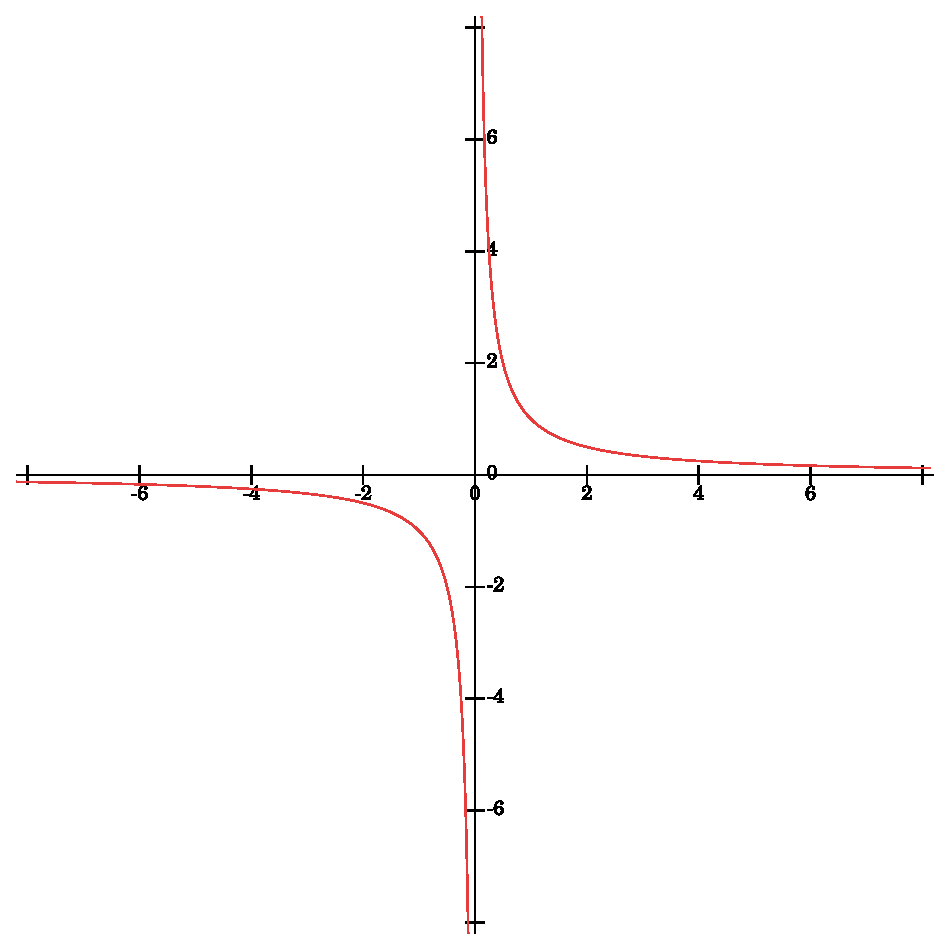
\includegraphics[height=6cm,width=6cm]{frecip.eps} 

\end{center}
\end{minipage}
\hfill
\newpage
\subsection{Gráfica de la función homográfica}

Para graficar la función homográfica mas fácilmente buscaremos transformar a esta \\
 en un corrimiento de la función reciproca:
\begin{center}

$f(x)= \dfrac{ax+b}{cx+d}$\\
$= \quad \langle$ factor común $a$ y $b$ $\rangle$\\
$f(x)=  \dfrac{ a \left( x + \dfrac{b}{a} \right) } 
			  { c \left( x + \dfrac{d}{c} \right) }$\\
$= \quad \langle$ sumo y resto $\dfrac{d}{c}$ $\rangle$\\
$f(x)=   \dfrac{a}{c} \times 
	    \dfrac{ x + \dfrac{d}{c} -\dfrac{d}{c} + \dfrac{b}{a}  } 
			  { x + \dfrac{d}{c}  }$\\

$= \quad \langle$ reparto $\dfrac{d}{c}$ $\rangle$\\
$f(x)=   \dfrac{a}{c} \times 
\left[
	    \dfrac{ x + \dfrac{d}{c}  } 
			  { x + \dfrac{d}{c}  }
+
	    \dfrac{ \dfrac{-d}{c} + \dfrac{b}{a}  } 
			  { x + \dfrac{d}{c}  }
\right]$\\
$= \quad \langle$ denominador común $\dfrac{d}{c}$ $\rangle$\\
$f(x)=   \dfrac{a}{c} \times 
\left[
	    1
+
	    \dfrac{ \dfrac{bc-da}{ca}   } 
			  { x + \dfrac{d}{c}  }
\right]$\\
$= \quad \langle$ resuelvo $\dfrac{d}{c}$ $\rangle$\\
$f(x)=   \dfrac{a}{c} \times 
\left[ 1 + \dfrac{bc-da}{ca \left(x + \dfrac{d}{c} \right)} \right]$\\					  
$= \quad \langle$ Distribuyo $\dfrac{a}{c}$ $\rangle$\\
$f(x)=  \dfrac{a}{c} + \dfrac{a}{c} \times 
\dfrac{bc-da}{ca \left(x + \dfrac{d}{c} \right)} $\\		
$= \quad \langle$ simplifico y resuelvo $\dfrac{a}{c}$ $\rangle$\\
$f(x)=  \dfrac{a}{c} + \dfrac{bc-da}{c^2 \left(x + \dfrac{d}{c} \right)} $\\
$= \quad \langle$ Separo expresiones $\dfrac{a}{c}$ $\rangle$\\
$f(x)=  \dfrac{a}{c} + \dfrac{bc-da}{c^2} \times \dfrac{1}{x + \dfrac{d}{c} } $\\	
$= \quad \langle$ Tomando a: $\dfrac{a}{c}=v$; $\dfrac{bc-da}{c^2}=u$; $\dfrac{-d}{c}=w$ \quad nos queda: $\rangle$\\
\qquad \\
$\dfrac{u}{x-w}+v$\\
\qquad \\
Esto es la función reciproca corrida horizontalmente $w$ unidades, verticalmente $v$ unidades y expandida, contraída o reflejada, verticalmente según $u$.
		  
\end{center}

\newpage
\subsection{Raíces de la homográfica}

Como se muestra las raíces son las mismas que las raíces del polinomio numerador:

$$f(x)= 0 \Leftrightarrow \dfrac{ax+b}{cx+d}=0 \Rightarrow ax+b = 0 \Leftrightarrow x = \dfrac{-b}{a}$$

\subsection{Intersección con el eje $Y$}
$$f(0) = \dfrac{a\times 0+b}{c\times 0+d}
= \dfrac{b}{d}$$
\subsection{Asíntotas}

• La asíntota vertical es el corrimiento vertical: $\dfrac{-d}{c} = w$

• La asíntota horizontal es el corrimiento horizontal: $\dfrac{a}{c} = v$

\subsection{Dominio e Imagen}

• Dominio: $\mathbb{R}\smallsetminus \left\{\dfrac{-d}{c}\right\} =
\mathbb{R}\smallsetminus \{w\} $

• Imagen: $\mathbb{R}\smallsetminus \left\{\dfrac{a}{c}\right\} = 
\mathbb{R}\smallsetminus \{v\}$

\subsection{Otra forma: Ejemplo}

Usaremos la función simple $f(x)=\dfrac{x+1}{x-1}$\\
\hfill
\quad \\
\quad \\
\begin{minipage}{.30\textwidth}

\paragraph{• Forma 1}
\quad \\
Es el método desarrollado \\
anteriormente:
\\
\begin{center}
$ \dfrac{x+1}{x-1}$\\
$= \quad \langle$ sumo y resto 1  $\rangle$\\
$ \dfrac{x+1+1-1}{x-1}$\\
$= \quad \langle$ reparto  $\rangle$\\
$ \dfrac{x-1}{x-1}+\dfrac{1+1}{x-1}$\\
$= \quad \langle$ resuelvo  $\rangle$\\
$ \dfrac{2}{x-1}+1$\\
\end{center}
\end{minipage}
\hfill
\begin{minipage}{.55\textwidth}
\paragraph{• Forma 2}
La segunda forma consta en realizar la división de polinomios y hacer uso de:\\
\begin{center}
$\dfrac{dividendo}{divisor}=cociente \times divisor +resto \Leftrightarrow $\\
$ \Leftrightarrow  dividendo= divisor \times \left(cociente+\dfrac{resto}{divisor}\right) \Leftrightarrow $\\
$\Leftrightarrow \dfrac{dividendo}{divisor}=cociente+\dfrac{resto}{divisor}$\\
\quad \\

\end{center}

\hfill
\begin{minipage}{.45\textwidth}
$
\begin{array}{c|c}
 x + 1 & x - 1 \\
\hline 
- \qquad \qquad & 1 \qquad \\
 x-1 &\\
\hline 
 \smallsetminus \quad 2 &
\end{array}$\\
\end{minipage}
\hfill
\begin{minipage}{.45\textwidth}
\begin{center}

Resultando:
$$\dfrac{x+1}{x-1} = \dfrac{2}{x-1}+1$$
\end{center}
\end{minipage}
\hfill
\\
\end{minipage}
\hfill \\
\quad \\


• La asíntota vertical es el corrimiento vertical: $\dfrac{-(-1)}{1} = 1$

• La asíntota horizontal es el corrimiento horizontal: $\dfrac{1}{1} = 1$

• Dominio: $\mathbb{R}\smallsetminus \left\{\dfrac{-(-1)}{1}\right\} =
\mathbb{R}\smallsetminus \{1\} $

• Imagen: $\mathbb{R}\smallsetminus \left\{\dfrac{1}{1}\right\} = 
\mathbb{R}\smallsetminus \{1\}$

• Raices: $\dfrac{x+1}{x-1} =0 \Rightarrow x+1=0 \Leftrightarrow x=-1$

• Intersección con el eje $Y$: $f(0) = \dfrac{0+1}{0-1} = -1$

Grafica:\\
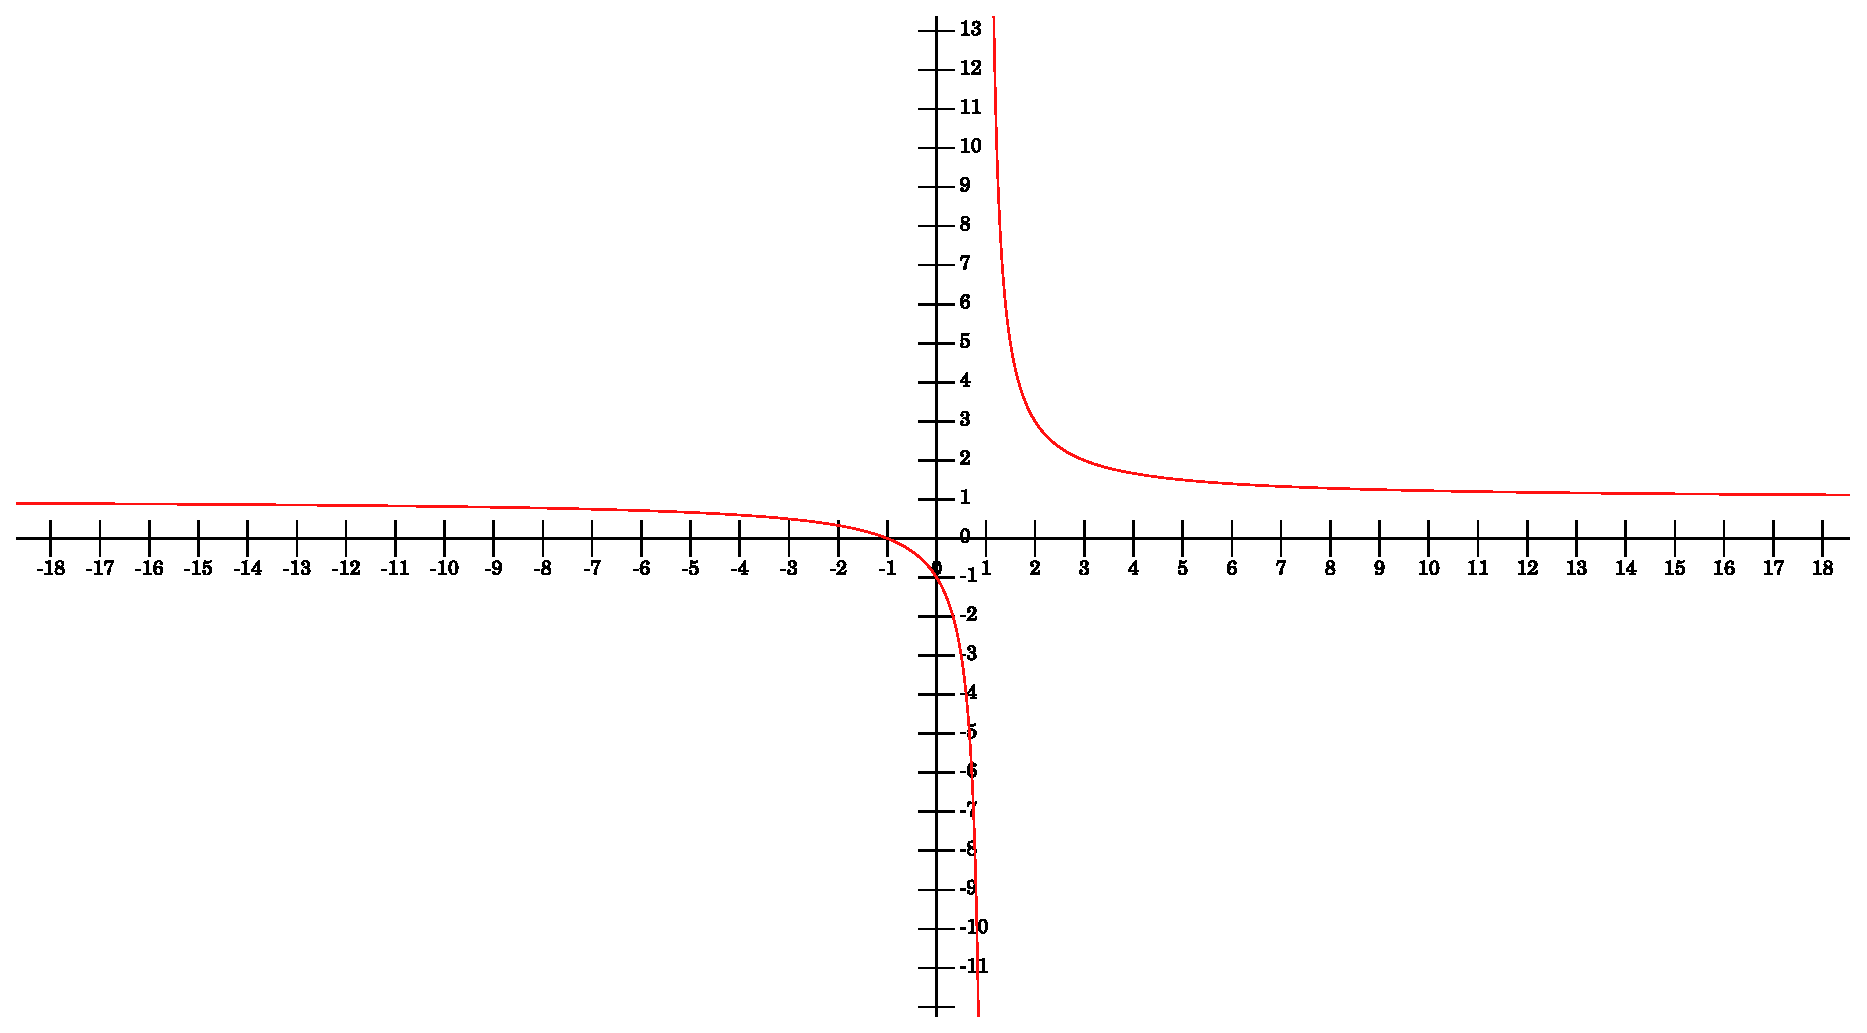
\includegraphics[height=8cm,width=14cm]{hipej.eps} 

\section{Funciones Trigonométricas}
\paragraph{Trigonométrica}
\quad \\
\quad \\
\hfill
\begin{minipage}{.30\textwidth}
Circunferencia trigonométrica
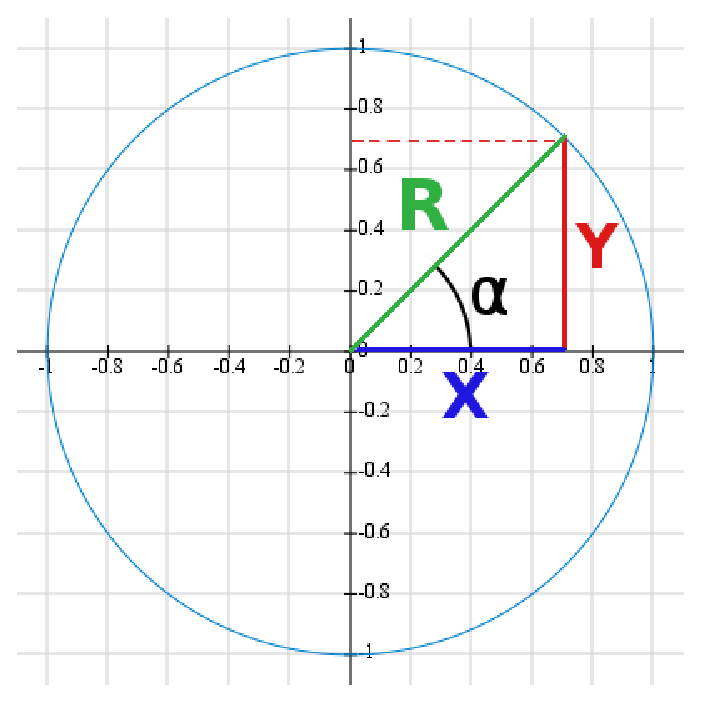
\includegraphics[height=4cm,width=4cm]{ct.eps} 
\end{minipage}
\hfill
\begin{minipage}{.20\textwidth}
$\textbf{R}=1$\\
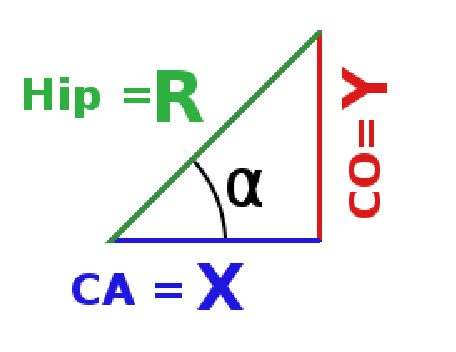
\includegraphics[height=2.5cm,width=3cm]{tt.eps} 

\end{minipage}
\hfill
\begin{minipage}{.40\textwidth}
\begin{center}
$
\begin{array}{ccc}

seno (\alpha) & = & \dfrac{CO}{H} = \dfrac{Y}{R} \\
\\
coseno (\alpha) & = & \dfrac{CA}{H} = \dfrac{X}{R} \\
\\
tangente (\alpha) & = & \dfrac{CO}{CA} = \dfrac{O}{A} = \dfrac{Y}{X} \\
\end{array}$\\
\end{center}
\end{minipage}
\hfill
\subsection{Función Seno}

Sea $f: \mathbb{R} \longrightarrow \mathbb{R} / f(x)= sen(x)$ \\

Nuestro objetivo, ademas de estudiar esta función es esposar su gráfica. Para lo cual comenzaremos viendo algunas características destacadas.\\

• $-1 \leq sen(x) \leq 1$ $\forall x \in \mathbb{R}$\\

\qquad $\therefore $ Im$f = [-1,1]$

\qquad luego Gr$f$ esta entre las rectas $y=-1$ e $y=1$.\\

• $sen(x) = -sen(x) \Rightarrow $ es impar $\Rightarrow$ Gr$f$ es simétrica respecto del origen de coordenadas.\\

• $sen(x+2 \pi) = sen(x)$ $ \forall x \in \mathbb{R}$\\

\qquad $\therefore$ $f$ es periódica de periodo $2\pi$.\\

\qquad Conociendo la gráfica en $(0, \pi)$, se conoce en todos los $\mathbb{R}$\\

• $sen(\pi -x) = sen(x)$\\

• $sen(\pi +x) = -sen(x)$\\
\\
Con estas ayudas y con la circunferencia trigonométrica terminaremos la Gr$(sen)$.
\paragraph{Gráfica de la función seno}
\begin{center}
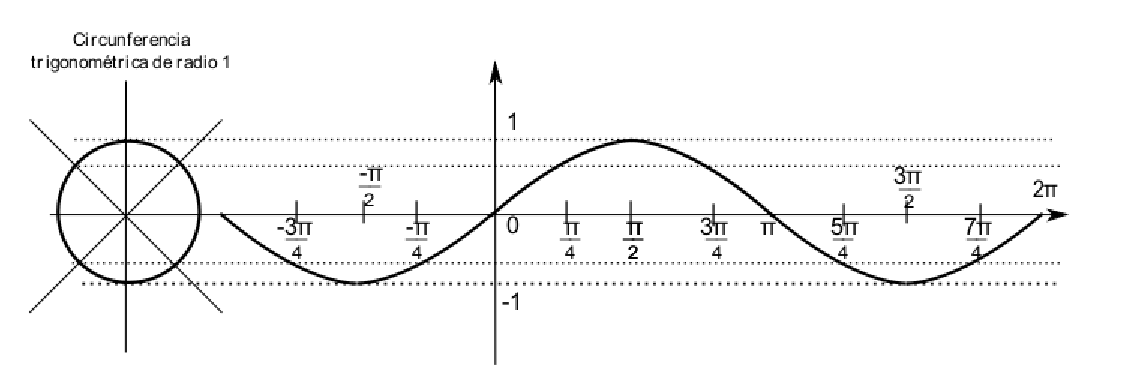
\includegraphics[height=5cm,width=15cm]{sen.eps} 
\end{center}

\paragraph{Raices}
\qquad\\

Notemos que: $f(x)=0 \Leftrightarrow x= k \pi$ $/$ $k\in \mathbb{Z}$
\subsection{Función Coseno}

Sea $f: \mathbb{R} \longrightarrow \mathbb{R} / f(x)= cos(x)$ \\

Podriamos trabajar como con la función seno y llegar a la gráfica a través de la circunferencia trigonométrica. Pero optaremos por hacerlo utilizando la siguientes propiedades:\\

• $cos(x)=cos(-x)$ la función es par.\\

• $cos(x) = cos(-x) = sen \left(\dfrac{\pi}{2} -(-x)\right) = sen \left(\dfrac{\pi}{2} + x \right)$ \quad $\forall x \in \mathbb{R}$\\

\paragraph{Gráfica de la función coseno}
\begin{center}
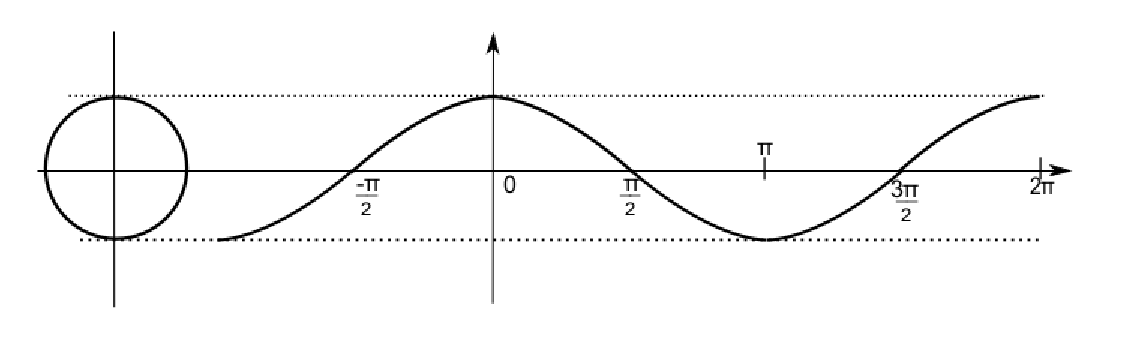
\includegraphics[height=4.3cm,width=15cm]{cos.eps} 
\end{center}

\paragraph{Raices}
\qquad\\

Notemos que: $f(x)=0 \Leftrightarrow x= \dfrac{\pi}{2} + k \pi$ $/$ $k\in \mathbb{Z}$
\subsection{Función Tangente}

Sea $f: D \longrightarrow \mathbb{R} / f(x)= tg(x)$ \\

\qquad $D = \left\{
 x \in \mathbb{R} / x \neq \dfrac{2k+1}{2} \times \pi ; k\in \mathbb{Z} \right\}$
 
\qquad \qquad $D$ es simétrico.

\paragraph{Propiedades:}


• $tg(x) = \dfrac{sen(x)}{cos(x)}$\\

• $tg(-x)=-tg(x)$ $\forall x \in D \Rightarrow$ es impar.\\

• $tg(x+\pi) = \dfrac{sen(x+\pi}{cos(x+\pi)}= \dfrac{-sen(x)}{-cos(x) = \frac{sen(x)}{cos(x)} }= tg(x)$\\
\qquad \qquad \qquad $\therefore$ $tangente$ es una función periódica de periodo $\pi$.
\paragraph{Grafica}
\begin{center}
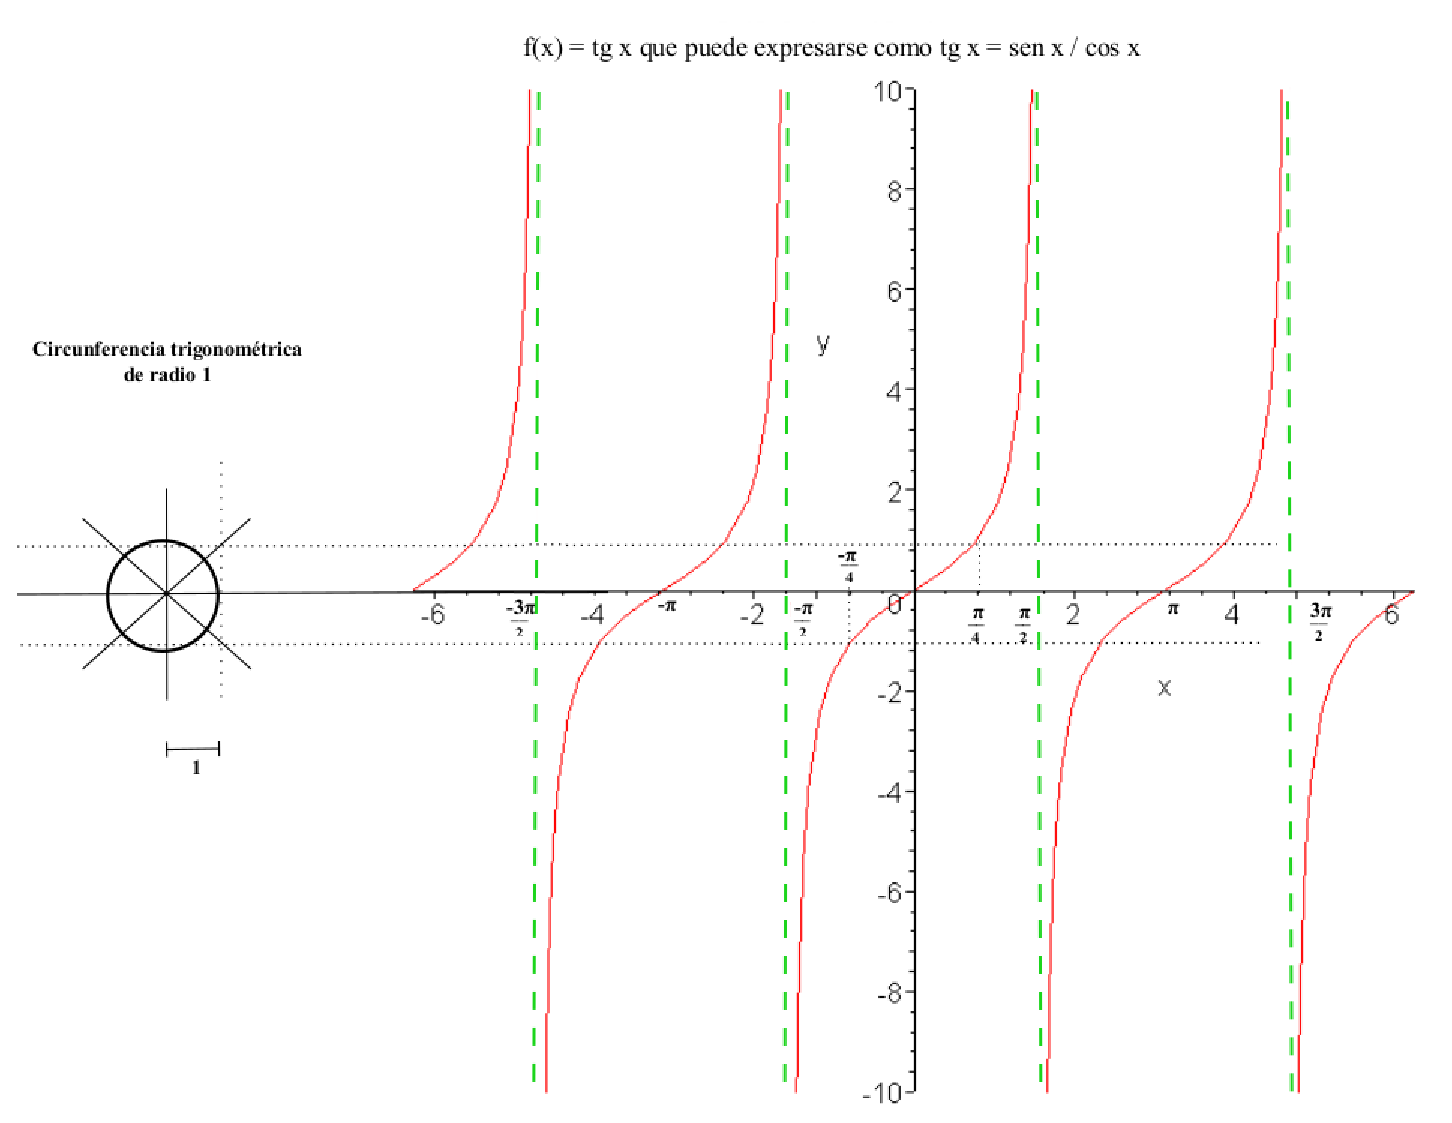
\includegraphics[height=10cm,width=14cm]{tg.eps} 
\end{center}

\subsection{Función Senoidal}

Sea $f: \mathbb{R} \longrightarrow \mathbb{R} / f(x)= c \times sen(kx+\alpha)$  \quad Donde $c \neq 0$, $ k \neq 0$, $ \alpha $ son constantes $\in \mathbb{R}$\\

\paragraph{Propiedades}

• Dom$f = \mathbb{R}$\\

• Im$f = [c, -c]$\\

• $f$ es periódica de periodo $\dfrac{2\pi}{k}$, ya que:\\

\qquad $f\left(x+\dfrac{2 \pi}{k}\right)= c \times sen\left(k \left(x+\dfrac{2 \pi}{k}\right)+\alpha \right) \Rightarrow c \times sen(kx+2\pi+\alpha) \Rightarrow c \times sen(kx+\alpha +2\pi) \Leftrightarrow$\\

\qquad $\Leftrightarrow c\times sen(kx+\alpha)=f(x)$\quad $\forall x \in \mathbb{R}$

\paragraph{Gráfica}
\qquad \\

Se suele transformar la ecuación de la función para poder transformarla en corrimiento de alguna función ya conocida. En este caso vamos a proceder de la siguiente forma para lograr una función seno corrida.\\

Primero transformamos la función ligeramente:
\begin{center}
$
\begin{array}{ccc}

f(x) & = & c \times sen(kx+\alpha)\\
= \langle factor &  comun &\rangle \qquad \qquad\\
f(x) & = & c \times sen\left(k\left(x+\dfrac{\alpha}{k}\right) \right)\\
\end{array}$\\
\end{center}
Y luego graficamos por corrimientos:
\begin{center}
$
\begin{array}{ccc}

f_1(x) & = & sen(x)\\
f_2(x) & = &c \times sen(x)\\
f_3(x) & = &c \times sen(kx)\\
f(x) & = &c \times sen\left(k\left(x+\dfrac{\alpha}{k}\right) \right)
\end{array}$\\

\end{center}

\paragraph{Ejemplo}

\qquad $f(x)  = 3 \times sen(5x+1)$

\hfill
\begin{minipage}{.45\textwidth}
• Dom$f = \mathbb{R}$\\
• Im$f = [3, -3]$\\
• $f$ es periódica de periodo $\dfrac{2\pi}{5}$ \\
\\

Primero transformamos la función ligeramente:
\begin{center}
$\begin{array}{ccc}
f(x) & = & 3 \times sen(5x+1)\\
f(x) & = & 3 \times sen \left(5\left(x+\dfrac{1}{5}\right) \right)\\
\end{array}$\\
\end{center}

Y luego graficamos por corrimientos:


\begin{center}

$
\begin{array}{ccc}

f_1(x) & = & sen(x)\\
f_2(x) & = &3 \times sen(x)\\
f_3(x) & = &3 \times sen(5x)\\
f(x) & = &3 \times sen\left(k\left(x+\dfrac{\alpha}{k}\right) \right)
\end{array}$\\
\end{center}


\end{minipage}
\hfill
\begin{minipage}{.45\textwidth}

Grafica de  $f_1$: roja; $f_2$: azul; $f_3$:verde. \\
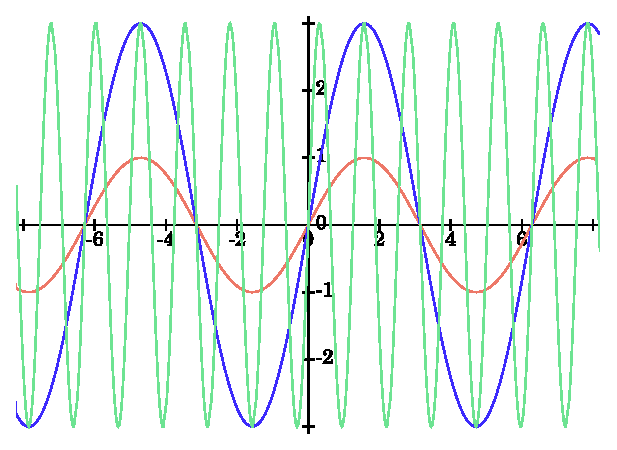
\includegraphics[height=4cm,width=8cm]{fsnd1.eps} \\

Grafica de  $f(x)=3 \times sen\left(k\left(x+\dfrac{\alpha}{k}\right) \right)$ \\
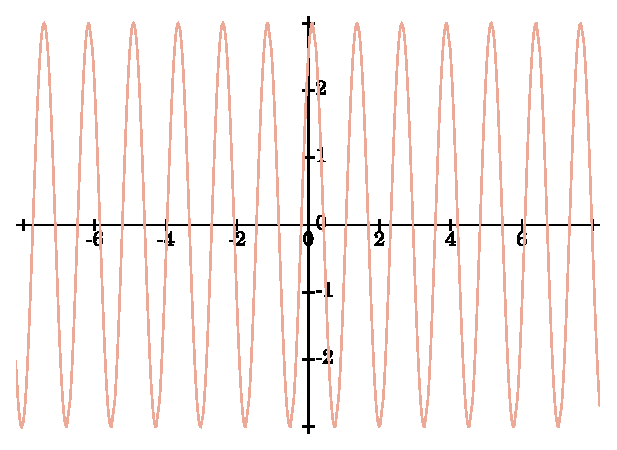
\includegraphics[height=4cm,width=8cm]{fsnd2.eps} \\

\end{minipage}
\hfill
\newpage
\section{Composición de funciones}

\hfill
\begin{minipage}{.45\textwidth}
La composicion de funciones es una operación mas entre dos funciones.\\

Sean dos funciones reales $f$ y $g$.
$$f:D_1\longrightarrow C_1 \qquad \qquad g: D_2 \longrightarrow C_2$$

\end{minipage}
\hfill
\begin{minipage}{.45\textwidth}
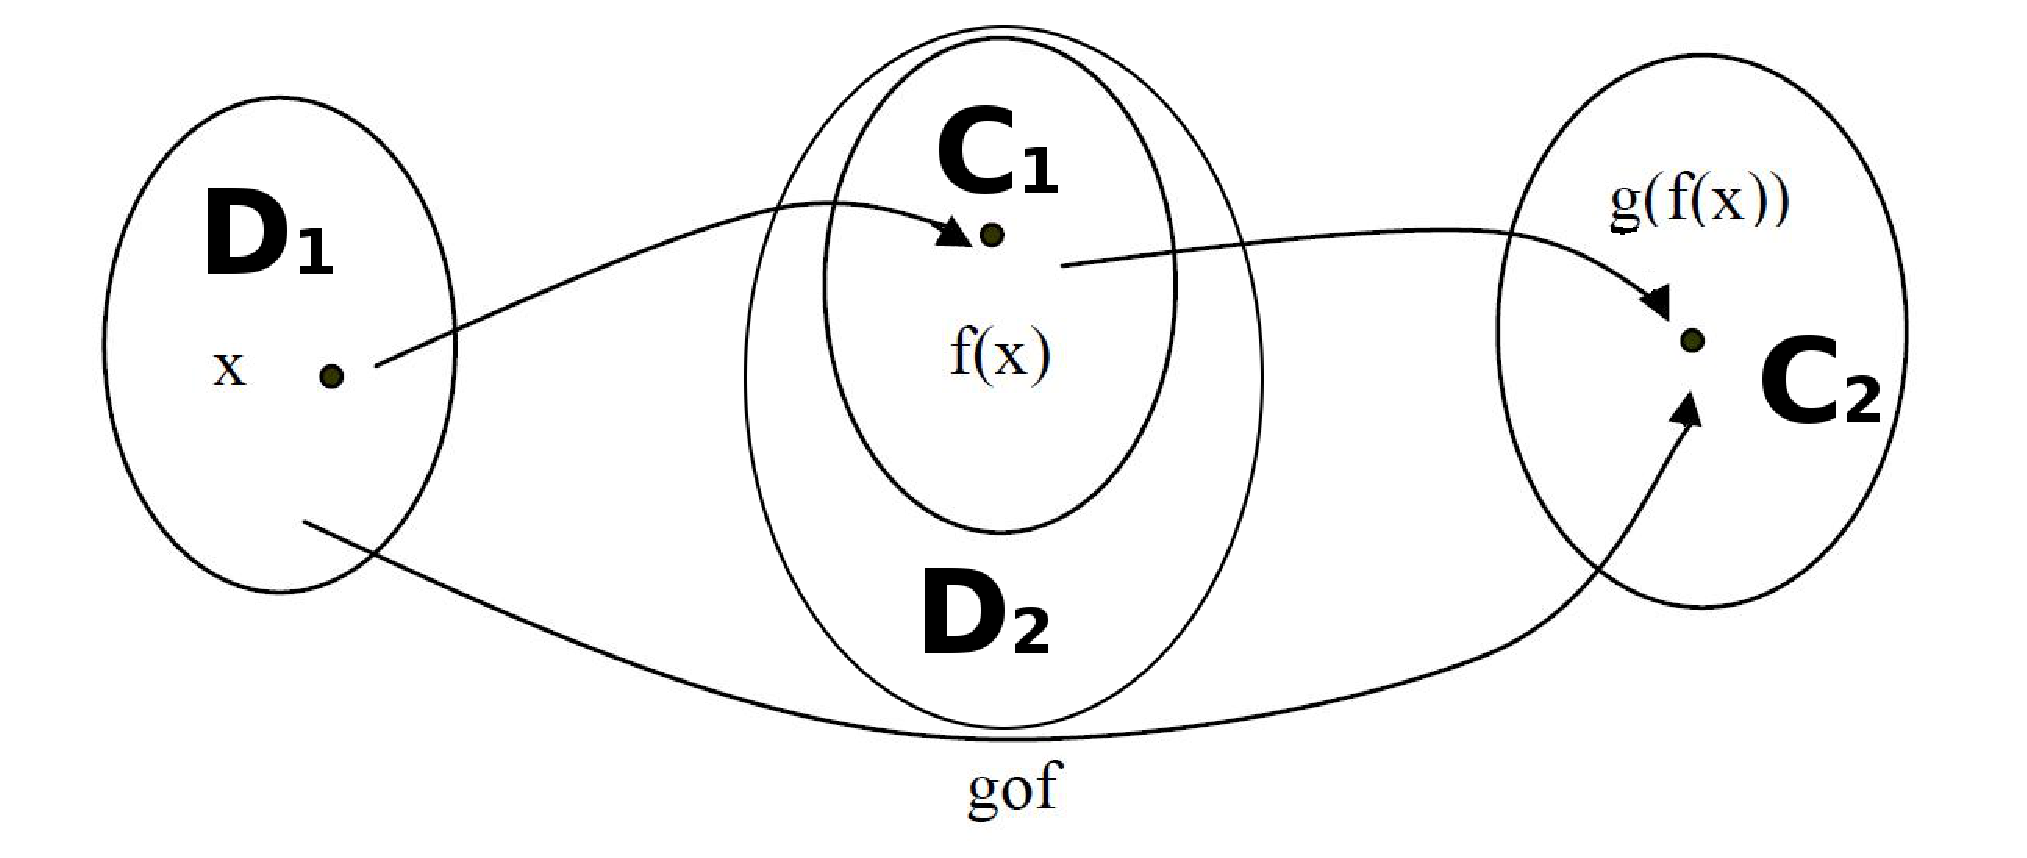
\includegraphics[height=4cm,width=8cm]{cnmpp.eps} 
\end{minipage}
\hfill

Llamaremos función compuesta a la definida por:
\begin{center}
$g\circ f:D\longrightarrow C/$\\
$ $\qquad $ $ \qquad $ $ \qquad $x \longrightarrow (g\circ f)_{(x)}=g(f(x))$\\
\qquad\\
Donde: Dom$(g\circ f) = \{x \in $ Dom$f$ $/$ $f(x) \in $ Dom$g\}$\\
\end{center}

\paragraph{Ejemplo}
$g\circ f$\\
\\
$
\begin{array}{ccccc}

    & &f(x)=x^2-x-1 & & g(x)=\dfrac{1}{x}\\
 \\
Dom & & \mathbb{R} & & \mathbb{R}\smallsetminus\{0\} \\

\end{array}$\\
\\

Por lo tanto el Dom$(f\circ g)$ sera:
\\

\hfill
\begin{minipage}{.45\textwidth}
\begin{center}
$\{ x \in \mathbb{R} / f(x) \in \mathbb{R}\smallsetminus \{o\}\} \Leftrightarrow $\\
\qquad\\

$\Leftrightarrow \{ x \in \mathbb{R} / x^2-x-1 \in \mathbb{R}\smallsetminus \{o\}\} \Leftrightarrow $\\
\qquad\\

$\Leftrightarrow \left\{ x \in \mathbb{R} / x \in \mathbb{R}\smallsetminus \left\{\dfrac{1-\sqrt{5}}{2}, \dfrac{1+\sqrt{5}}{2}\right\}\right\} $\\

\end{center} 
\end{minipage}
\hfill
\begin{minipage}{.45\textwidth}
$$x^2-x-1 \neq 0 \Leftrightarrow x\neq \dfrac{1+\sqrt{5}}{2} \vee x\neq \dfrac{1-\sqrt{5}}{2}$$
\end{minipage}
\hfill\\
\\

Buscamos la ley:

\qquad $(g\circ f)_{(x)} = g(f(x) =g(x^2-x-1) = \dfrac{1}{x^2-x-1}$\\

En conclusión nuestra función es:

\begin{center}
$
g\circ f: \mathbb{R} \smallsetminus \left\{ \dfrac{1- \sqrt{5}}{2}, \dfrac{1+ \sqrt{5}}{2}\right\}  \longrightarrow \mathbb{R}$\\
$ $\qquad $ $ \qquad $ $ \qquad $x \longrightarrow (g\circ f)_{(x)}= \dfrac{1}{x^2-x-1}$\\
\qquad\\

\end{center}

\section{Función Inyectiva}

Sea $f : D \longrightarrow C$ una funcion real.\\

Decimos que  $f$ es una ``función inyectiva'' sii $\forall x_1, x_2 \in D$, con $x_1 \neq x_2 \Rightarrow f(x_1) \neq f(x_2)$, o su equivalente:
$$f(x_1)=f(x_2) \Rightarrow x_1=x_2$$ 

\paragraph{Ejemplo}

\qquad \textbf{1)} $f(x)=x^2-1$ no es inyectiva pues:

\begin{center}
$-1,1 \in $ Dom$f$ $ -1 \neq 1 \wedge $ $f(1)=f(-1)=0$ 
\end{center}

\qquad \textbf{2)} $g(x)=2x-3$ es inyectiva pues:\\

Sean $x_1$, $x_2$ $\in$ Dom$g$.
\begin{center}
$ g(x_1)=g(x_2) \Leftrightarrow 2x_1-3=2x_2-3 \Leftrightarrow 2x_1=2x_2 \Leftrightarrow
x_1 = x_2$
\end{center}

\section{Función Sobreyectiva}

Sea $f:D \longrightarrow C$ un función real.\\

Decimos que $f$ es una ``función sobreyectiva o suryectiva'' sii:
\begin{center}
Cod$f = $ Im$f$
\end{center}

\paragraph{Ejemplos}
\qquad \\

\qquad \textbf{1)} 

\hfill
\begin{minipage}{.45\textwidth}
\begin{center}
$f: \mathbb{R} \longrightarrow \mathbb{R}$\\
$ $ \qquad $ $ \qquad $ $ \qquad $ $ \qquad $ x \longrightarrow f(x) = x^2$\\
\end{center}
\end{minipage}
\hfill
\begin{minipage}{.45\textwidth}
$\left.
\begin{array}{ccc}
Cod(f)&=& \mathbb{R}\\
Im(f) &=& \mathbb{R} _0 ^+\\
\end{array}\right\} \Rightarrow
 Cod(f) \neq Im(f)$\\
\end{minipage}
\hfill\\
\begin{center}
$\therefore$ no es sobreyectiva.
\end{center}

\qquad \textbf{2)} \\


\hfill
\begin{minipage}{.45\textwidth}
\begin{center}
$f: \mathbb{R} \longrightarrow \mathbb{R} _0 ^+$\\
$ $ \qquad $ $ \qquad $ $ \qquad $ $ \qquad $ x \longrightarrow f(x) = x^2$\\
\end{center}
\end{minipage}
\hfill
\begin{minipage}{.45\textwidth}
$\left.
\begin{array}{ccc}
Cod(f)&=& \mathbb{R}\\
Im(f) &=& \mathbb{R} _0 ^+\\
\end{array}\right\} \Rightarrow
 \mathbb{R} _0 ^+ = \mathbb{R} _0 ^+$\\
\end{minipage}
\hfill\\
\begin{center}
$\therefore$ es sobreyectiva.
\end{center}

\section{Función Biyectiva}

Sea $f$ una función real. Diremos que $f$ es una ``función biyectiva'' sii $f$ es inyectiva y sobreyectiva.\\

\paragraph{Ejemplo}
\qquad\\

\qquad Sea $f: \mathbb{R} \longrightarrow \mathbb{R}$ $/$ $f(x)=5x$\\

\qquad • es inyectiva, en efecto:
$$x_1 \neq x_2 \Rightarrow 5x_1 \neq 5x_2 \Rightarrow f(x_1) \neq f(x_2)$$

\qquad • es sobreyectiva pues:\\

\qquad \qquad ¿$\exists x$, Dom$f= \mathbb{R}$ $/$ $f(x)=y$?\\

\hfill
\begin{minipage}{.45\textwidth}
\begin{center}
$f(x)=y$\\$x=\dfrac{y}{5}$\\
$5x=y$
\end{center}
\end{minipage}
\hfill
\begin{minipage}{.45\textwidth}
$\therefore$ dado $y \in $ Cod$f$\\

\qquad \qquad $ \exists \dfrac{y}{5} \in \mathbb{R}$ $/$ $f\left(\dfrac{y}{5}\right)=y$\\

\qquad \qquad \qquad Osea: $y \in \mathbb{R}$ y $\dfrac{y}{5} \in \mathbb{R}$ 
\end{minipage}
\hfill
\begin{center}
Luego es biyectiva.
\end{center}

\paragraph{Nota}
: para determinar si $f$ es sobre hay que despejar $x$ y ver que $y$ pueda tomar cualquier valor de Cod$f$.

En el ejemplo anterior esto se lleva a cabo probando $y \in \mathbb{R}$ y $\dfrac{y}{5} \in \mathbb{R}$.
\section{Funcion Inversa}

Sea $f: D \longrightarrow C$ una función real biyectiva.\\

\quad Llamaremos ``función  inversa'' de $f$ y la notaremos $f^{-1}$ a la función definida por:
\begin{center}
$f^{-1}: C \longrightarrow D $\\
$ $ \qquad $ $ \qquad $ $ \qquad $ $ \qquad $ y \longrightarrow f^{-1}(y) = x$ $/$ $ y=f(x)$\\
\end{center}

\paragraph{Ejemplo}

\qquad $f: \mathbb{R} \longrightarrow \mathbb{R}$ $/$ $x \longrightarrow f(x)= 5x$

\qquad • Sabemos que $f$ es biyectiva $\Rightarrow \exists$ $f^{-1} : \mathbb{R} \longrightarrow \mathbb{R}$ $/$ $y \longrightarrow f^{-1}(y)= \dfrac{y}{5}$
\subsection{Gráfica de la función inversa}

La grafica de una función y su inversa son simétricas respecto de la recta $y=x$, esto es:\\

\hfill
\begin{minipage}{.45\textwidth}
\begin{center}
$(a, b) \in $ Gr$(f) \Leftrightarrow f(a)=b \Leftrightarrow $\\
\qquad\\
$\Leftrightarrow a=f^{-1}(b) \Leftrightarrow (b, a) \in $ Gr$(f^{-1})$
\end{center}
\end{minipage}
\hfill
\begin{minipage}{.45\textwidth}
\begin{center}
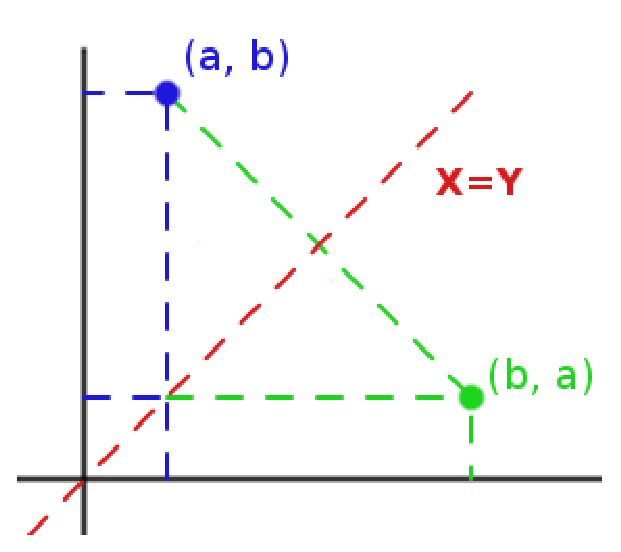
\includegraphics[height=2.5cm,width=4cm]{grffi.eps} \\
\end{center}
\end{minipage}
\hfill

\subsection{Propiedad}
\hfill
\begin{minipage}{.45\textwidth}
\begin{center}
$$f\circ f^{-1} = id $$
\end{center}
\end{minipage}
\hfill
\begin{minipage}{.45\textwidth}
\begin{center}
$$f^{-1}\circ f = id $$
\end{center}
\end{minipage}
\hfill \\

\textbf{Nota:} Existen casos en que esta propiedad no se cumplen, como $g(x)=x^2$.\\

\qquad Ya que no se cumpliría $f^{-1}\circ f = id $ es decir $\sqrt{x^2}=|x| \neq x$,

\qquad \quad solo se cumpliría si restringimos el dominio para los $\mathbb{R} _0 ^+$.
\section{Función Exponencial}

Sea $f(x)= a^x$\qquad $a>0 $ $\wedge$ $ a\neq 1$ \\

\qquad Llamemos a $f$ función exponencial.

• Analisemos:\\

\textbf{1)} Si $x=n$ \quad $n \in \mathbb{N}$ entonces $a^x=a^n=a_0 \times a_1 \times \cdots \times a_n$\\

\textbf{2)} Si $x=0$ \quad $a^0 =1$\\

\textbf{3)} Si $x\in \mathbb{Q}$ \quad $\Rightarrow \dfrac{p}{q}$ \quad $p,q \in \mathbb{Z}$, $q \neq 0$
$$a^x=a^{^p/_q}=\sqrt[q]{a^p}$$

\textbf{4)} Si $x \in \mathbb{Z} ^+ \Rightarrow x =n$ \quad $n \in \mathbb{N}$ $\therefore$ $a^x=a^n$\\ 

\textbf{5)} Si $x \in \mathbb{Z} ^- \Rightarrow x =-n$ \quad $n \in \mathbb{N}$ $\therefore$ $a^x=a^{-n}=\dfrac{1}{a^n}$\\

\textbf{6)} Si $x \in \mathbb{R}$ caso general.\\

\qquad No estamos en condiciones de definir con precision potencias de exponente irracional, pero no tenemos problemas en generalizar nuestros resultados.\\

\paragraph{Propiedades}
\qquad \\

• Dom$f = \mathbb{R}$ \qquad • Im$f= \mathbb{R}^0$\\

• Propiedades:\\

\quad	Dados $n,m,x,y \in \mathbb{R}$\\

\hfill
\begin{minipage}{.45\textwidth}


\textbf{1)} $ a^n \times a^m = a^{n+m}$\\
\textbf{2)} $\dfrac{a^n}{a^m} = a^{n-m}$

\end{minipage}
\hfill
\begin{minipage}{.45\textwidth}


\textbf{3)} $ (ab)^x = a^x \times b^x$\\
\textbf{4)} $(a^x)^y = a^{xy}$

\end{minipage}
\hfill \\
\qquad \\

\textbf{5)} Si $0 <a <b$ $\Rightarrow
\left\{
\begin{array}{ccc}
a^x<b^x & si & x>0 \\
a^x > b^x & si & x<0\\
\end{array}\right.$

\subsection{Función exponencial en general}

Si $f(x)=a^x$ \qquad $f(x)>0$ \qquad $a>0 $ $\wedge$ $ a\neq 1$\\

\qquad • $f$ es inyectiva.\\

\qquad •  Si $a>1$ $\longrightarrow f$ es estrictamente creciente.

\qquad \quad Si $a<1$ $\longrightarrow f$ es estrictamente decreciente.\\

\qquad •  \textbf{y=0} es la asíntota horizontal.\\

\qquad •  La Gr$f$ corta al eje $Y$ en el punto $(0,1)$.\\

\qquad •  El punto $(1, a) \in $ Gr$f$.

\paragraph{Ejemplo $e^x$}

La funcion definida por $f(x)=e^x$\\

Donde $e$ es un numero irracional, cuyo nombre se debe a Leonard Euler (1727).\\
$$e \simeq 2,71828\ldots$$

\qquad •  $e>1$ la función es estrictamente creciente.\\

Mas precisamente como : $2<e<3 \Rightarrow
\left\{
\begin{array}{ccc}
2^x<e^x<3^x & si & x>0 \\
2^x > e^x >3^x & si & x<0\\
\end{array}\right.$


\paragraph{Gráfica de $e^x$}
\begin{center}

$e^x$ en rojo, $2^x$ en azul y $3^x$ en verde.\\
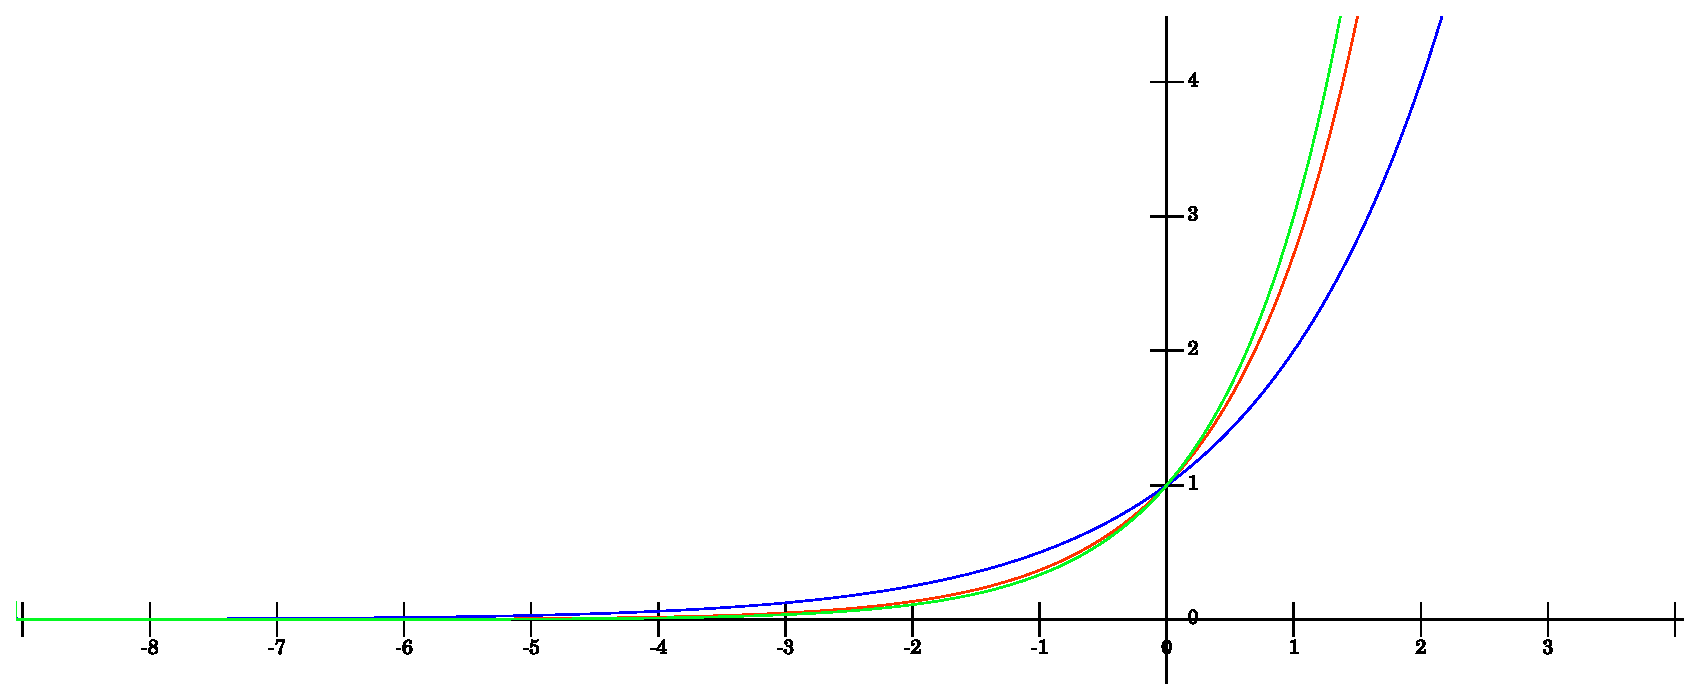
\includegraphics[height=6cm,width=16cm]{fexp.eps}

\end{center}

\section{Función Logarítmica}

Vimos que toda función exponencial\\
$$f(x)=a^x \qquad a>0\quad \wedge \quad a\neq 1$$
\qquad es inyectiva y por lo tanto admite función inversa, denominada ``función logarítmica de base $a$''.\\

La cual notamos de la siguiente forma: $\log _a y$

Y esta definida como:

\begin{center}
$f: \mathbb{R}^+ \longrightarrow \mathbb{R} $ $/$ \qquad $ $\\
$ $ \qquad $ $ \qquad $ $ \qquad $ $ \qquad $ y \longrightarrow \log _a y = x$ $ $ tal que $ a^x=y$\\
\end{center}
\qquad \qquad \textbf{Nota:} $\log _a y$ es el exponente al que hay que elevar ``a'' para obtener ``y''.

\paragraph{Ejemplos}
\qquad \\

\qquad $\log _3 81 = \textbf{4} \Leftrightarrow 3^{\textbf{4}} =81$\\

\qquad $\log _10 0,001= (\textbf{-3}) \Leftrightarrow 10^{(\textbf{-3})} = 0,001$\\

\subsection{Gráfica de $\log _a y$}

Sea $a>1$\\

\hfill
\begin{minipage}{.45\textwidth}
$a^x$ en rojo, $\log _a x$ en azul.\\
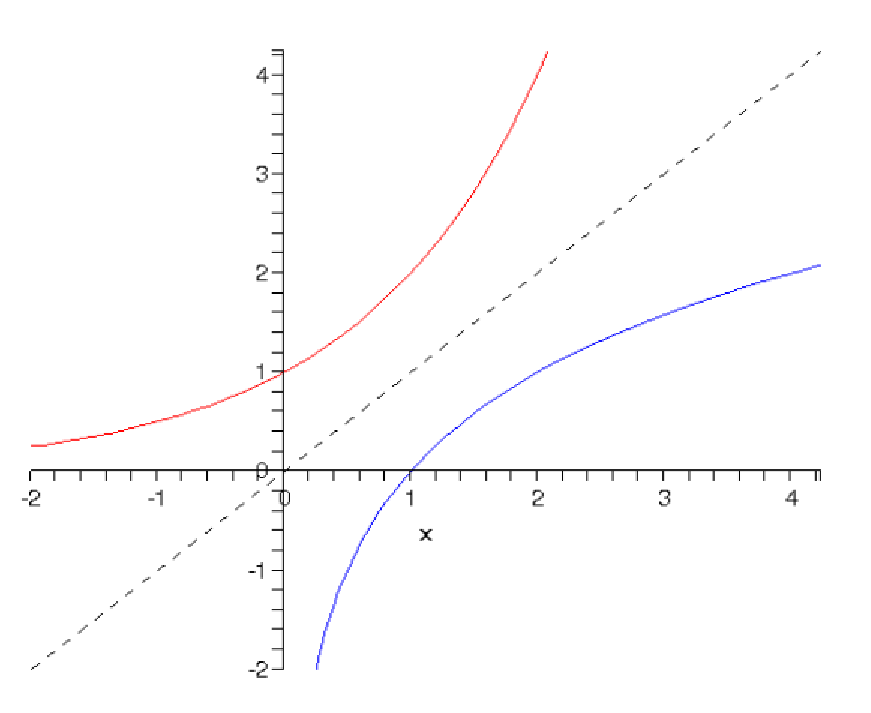
\includegraphics[height=6cm,width=6cm]{loga1.eps}

\end{minipage}
\hfill
\begin{minipage}{.45\textwidth}

• Dom$(\log _a) = \mathbb{R} ^+$ \\

• Im$(\log _a)= \mathbb{R}$\\

• $\log _a$ es una función estrictamente creciente.\\

• $x=0$ es asíntota vertical.

\end{minipage}
\hfill \\

Sea $a<1$\\

\hfill
\begin{minipage}{.45\textwidth}
$a^x$ en rojo, $\log _a x$ en azul.\\
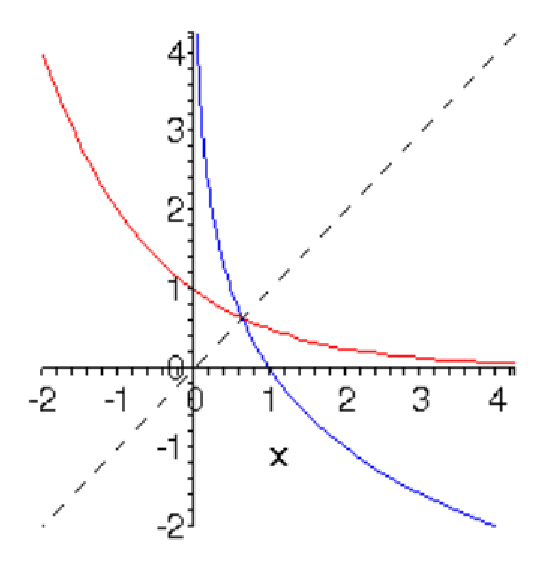
\includegraphics[height=6cm,width=6cm]{loga2.eps}
\end{minipage}
\hfill
\begin{minipage}{.45\textwidth}

• Dom$(\log _a) = \mathbb{R} ^+$ \\

• Im$(\log _a)= \mathbb{R}$\\

• $\log _a$ es  estrictamente decreciente.\\

• $x=0$ es asintota vertical.

\end{minipage}
\hfill \\

\paragraph{Notaciones}
\qquad \\

• Si $a=e$ entonces $\log _e x = \ln x$ (logaritmo neperiano o natural)\\

• Si $a=10$ entonces $\log _{10} x = \log x$

\subsection{Propiedades de $\log _a$}

$\forall a >1 \wedge a \neq 0$\\

\qquad \textbf{1)} $\log _a (xy) = \log _a x + \log _a y$\\

\qquad \quad \textbf{Demostración:}
\begin{center}
$\log _a (xy) = c \Leftrightarrow a^c = xy$\\
\qquad \\

$a^{\log _a (xy)} = a^{\log _a x + \log _a y} = a^{\log _a x} \times a^{\log _a y} \underset{a^{\log _a w}= w}{=} xy$\\

\qquad $\therefore$ $\log _a (xy) = \log _a x + \log _a y$
\end{center}

\qquad \textbf{2)} $\log _a \left(\dfrac{x}{y} \right) = \log _a x - \log _a y$\\

\qquad \textbf{3)} $\log _a x^y = y \log _a x$ \\

\qquad \quad \textbf{Demostración:}
\begin{center}
$x^y = a^{ y \log _a x}$\\
Es decir:\\
 $\log _a x^y = y \log _a x$\\
\end{center}

\subsection{Prop. Cambio de base $\log _a$}

$\forall a >1 \wedge a \neq 0$\\

$$\log _a x = \dfrac{\log _b x}{\log _b a} \quad, \qquad b>0$$

\quad \textbf{Demostración:}
\begin{center}
$y= \log _a x \Leftrightarrow a^y=x$\\
\qquad \\
$\log _b a^y \underset{a^y =x}{=} \log _b x \Leftrightarrow$\\
\qquad \\
$\underset{(3)}{\Leftrightarrow} y \log _b a = \log _b x \Leftrightarrow$\\
\qquad \\
$\Leftrightarrow y = \dfrac{\log _b x}{\log _b a}$\\
\qquad \\
$ $ \qquad $ $ \qquad $ $ \qquad $\therefore$ como $y=\log _a x $ concluimos: $\log _a x =  \dfrac{\log _b x}{\log _b a}$
\end{center}

\section{Funciones Hiperbólicas}

\subsection{seno hiperbólico}

La función seno hiperbólico esta definida como:

$$senh(x)=\dfrac{e^x-e^{-x}}{2}$$

• Dom$(senh) = \mathbb{R}$ \qquad  • Im$(senh) = \mathbb{R}$\\

• Es estrictamente creciente.\\

• $senh(-x) = \dfrac{e^{(-x)}-e^{-(-x)}}{2} = - \left[\dfrac{e^x-e^{-x}}{2} \right] = -senh(x)$ \qquad $\therefore$ $senh(x)$ es impar.

\paragraph{Gráfica}
\begin{center}
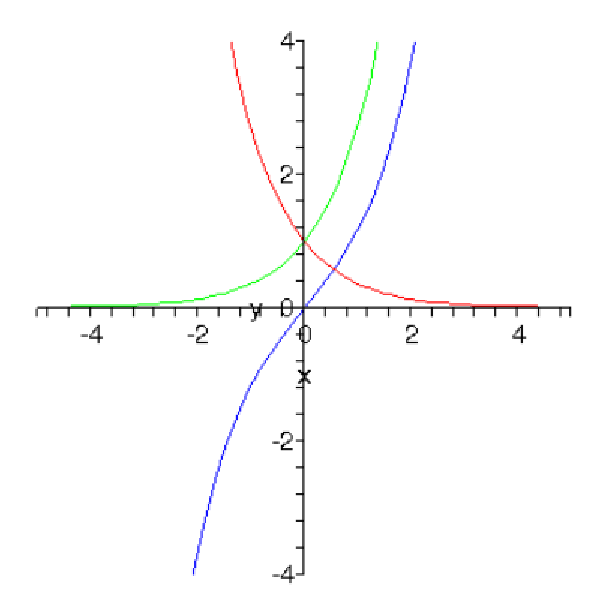
\includegraphics[height=6cm,width=6cm]{senh.eps}
\end{center}

\subsection{coseno hiperbólico}

La funcion coseno hiperbólico esta definida como:

$$cosh(x)=\dfrac{e^x+e^{-x}}{2}$$

• Dom$(cosh) = \mathbb{R}$ \qquad  • Im$(cosh) = [1,+\infty)$\\

• Es estrictamente: 

\qquad $ $\qquad $ $\qquad $ $\qquad $ $\qquad $ $ decreciente en $\mathbb{R} _0 ^-$

\qquad $ $\qquad $ $\qquad $ $\qquad $ $ \qquad $ $y creciente en $\mathbb{R} _0 ^+$.\\

• $cosh(-x) = \dfrac{e^{(-x)}+e^{-(-x)}}{2} = \dfrac{e^{-x}+e^x}{2} = cosh(x)$ \qquad $\therefore$ $cosh(x)$ es par.

\paragraph{Gráfica}
\begin{center}
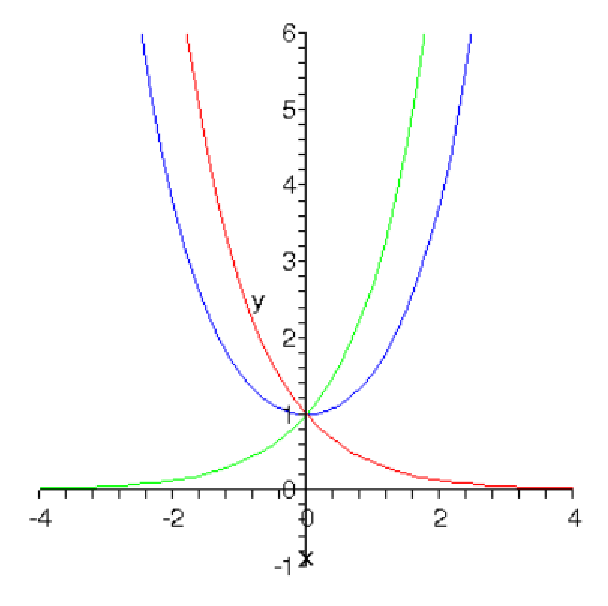
\includegraphics[height=6cm,width=6cm]{cosh.eps}
\end{center}

\subsection{tangente hiperbólica}

La funcion tangente hiperbólica esta definida como:

$$cosh(x) = \dfrac{senh(x)}{cosh(x)} = \dfrac{\dfrac{e^x-e^{-x}}{2}}{\dfrac{e^x+e^{-x}}{2}} = \dfrac{e^x-e^{-x}}{e^x+e^{-x}}$$

• Dom$(tgh) = \mathbb{R}$ \qquad  • Im$(tgh) = (-1, 1)$\\

• Es estrictamente creciente.\\

• $tgh(-x) =\dfrac{senh(-x)}{cosh8-x)}= \dfrac{-senh[x)}{cosh(x)} = -tgh(x) $\qquad $\therefore$ $tgh(x)$ es impar.

• Posee dos asíntotas horizontales: $y=1$ e $y=-1$

\paragraph{Gráfica}
\begin{center}
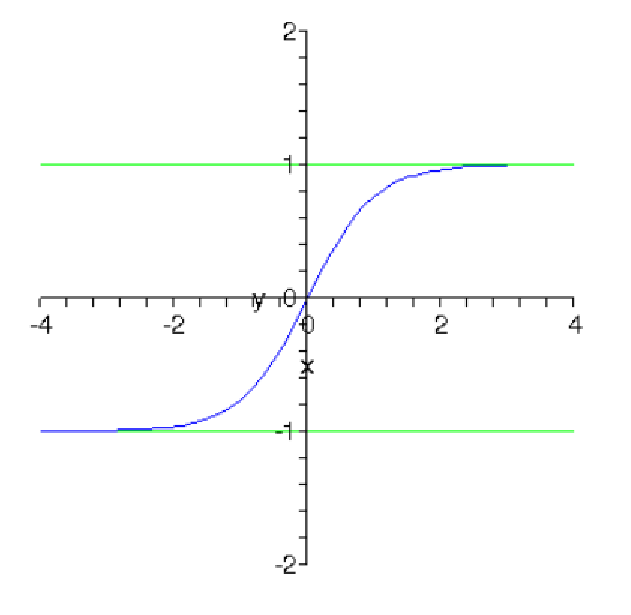
\includegraphics[height=6cm,width=6cm]{tgh.eps}
\end{center}

\subsection{Más funciónes hiperbólicas}

A partir de las funciónes anteriores se definen:

$$cosech(x)= \dfrac{1}{senh(x)}$$

$$sech(x)=\dfrac{1}{cosh(x)}$$

$$cotgh(x)=\dfrac{1}{tgh(x)}$$

\section{Funciones Trigonométricas inversas}

Sabemos que las funciónes trigonométricas estudiadas anteriormente, sen, cos y tg no son inyectivas debido a su periodicidad; pero podemos restringir su dominio a un intervalo donde si lo sean, y así hallar las funciones inversas de estas.

\subsection{arcseno}

\hfill
\begin{minipage}{.45\textwidth}

\begin{center}
$f:\left[ \dfrac{-\pi}{2},\dfrac{\pi}{2} \right] \longrightarrow [-1,1] $ $/$ \qquad $ $\\
$ $ \qquad $ $ \qquad $ $ \qquad $ $ \qquad $ x \longrightarrow f(x) = sen(x)$\\
\qquad \\

$f: [-1,1] \longrightarrow \left[ \dfrac{-\pi}{2}, \dfrac{\pi}{2} \right] $ $/$ \qquad $ $\\
$ $ \qquad $ $ \qquad $ y \longrightarrow f^{-1}(y) = x$ $/$ $ sen(x)=y$\\
\end{center}

\end{minipage}
\hfill 
\begin{minipage}{.50\textwidth}

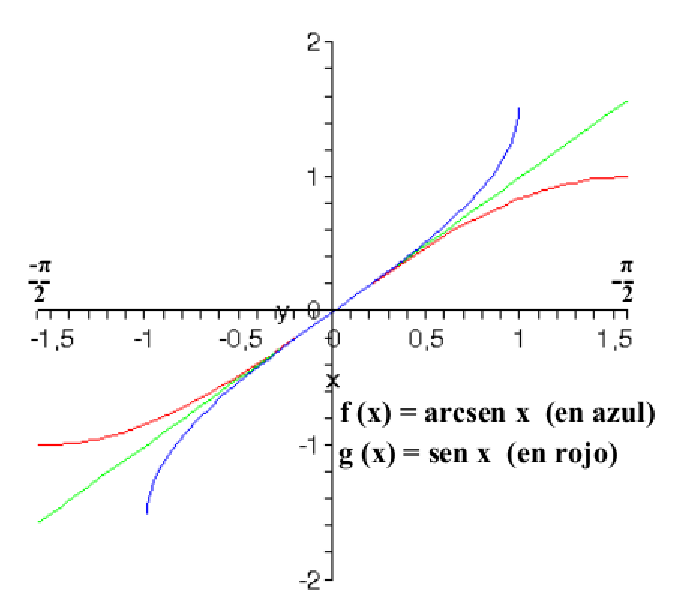
\includegraphics[height=6cm,width=6cm]{arcsen.eps}

\end{minipage}
\hfill \\

\subsection{arccoseno}

\hfill
\begin{minipage}{.45\textwidth}

\begin{center}
$f:[ 0, \pi] \longrightarrow [-1,1] $ $/$ \qquad $ $\\
$ $ \qquad $ $ \qquad $ $ \qquad $ $ \qquad $ x \longrightarrow f(x) = cos(x)$\\
\qquad \\

$f: [-1,1] \longrightarrow [0, \pi] $ $/$ \qquad $ $\\
$ $ \qquad $ $ \qquad $ y \longrightarrow f^{-1}(y) = x$ $/$ $ cos(x)=y$\\
\end{center}

\end{minipage}
\hfill 
\begin{minipage}{.50\textwidth}

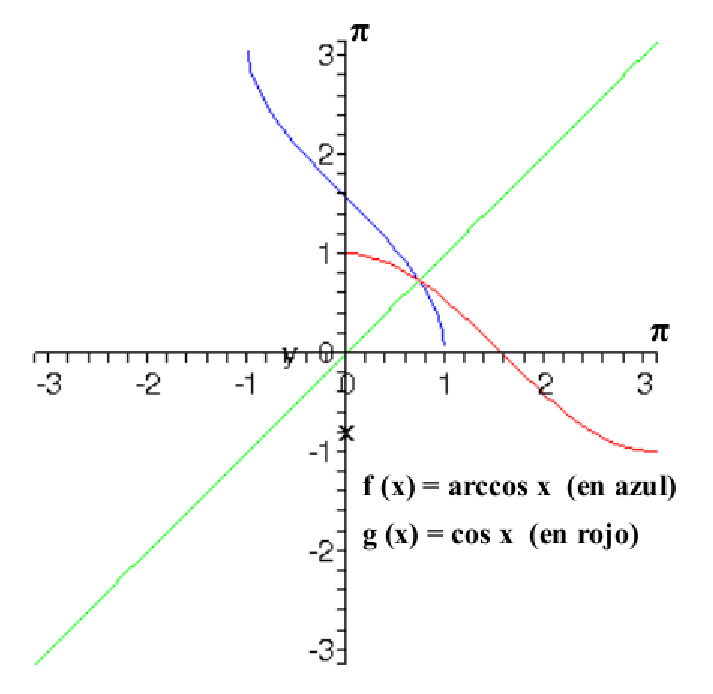
\includegraphics[height=6cm,width=6cm]{arccos.eps}

\end{minipage}
\hfill \\

\subsection{arctangente}

\hfill
\begin{minipage}{.40\textwidth}

\begin{center}
$f:\left[ \dfrac{-\pi}{2},\dfrac{\pi}{2} \right] \longrightarrow \mathbb{R} $ $/$ \qquad $ $\\
$ $ \qquad $ $ \qquad $ $ \qquad $ $ \qquad $ x \longrightarrow f(x) = tg(x)$\\
\qquad \\

$f: \mathbb{R} \longrightarrow \left[ \dfrac{-\pi}{2}, \dfrac{\pi}{2} \right] $ $/$ \qquad $ $\\
$ $ \qquad $ $ \qquad $ y \longrightarrow f^{-1}(y) = x$ $/$ $ tg(x)=y$\\
\end{center}

\end{minipage}
\hfill 
\begin{minipage}{.50\textwidth}

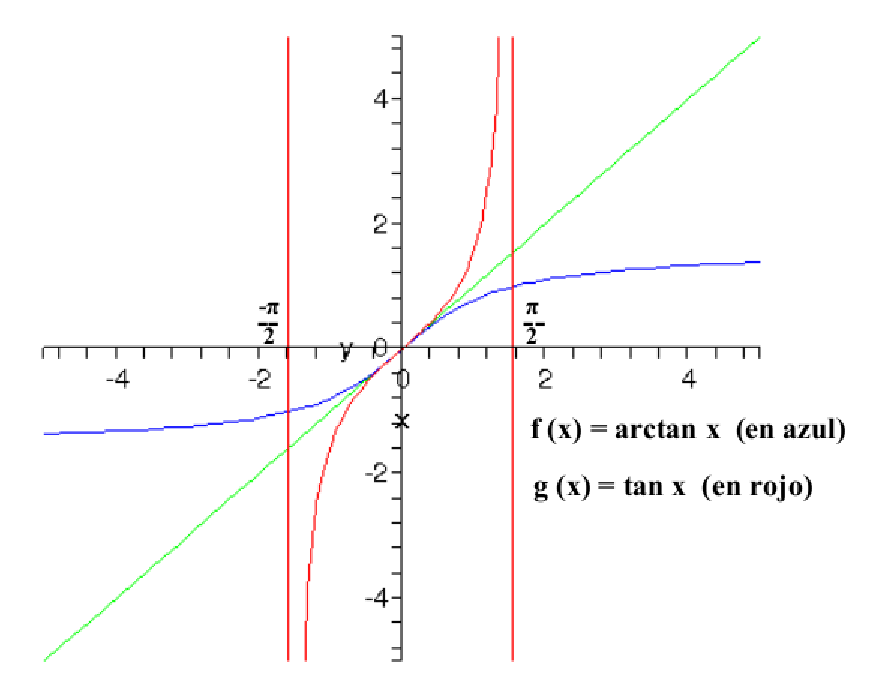
\includegraphics[height=6cm,width=8cm]{arctg.eps}

\end{minipage}
\hfill \\

\chapter{Limite y Continuidad}
\section{Limite}

El limite es la mayor erramienta para poder analisar el comportamiento de las funciones. \\
En si se trata de observar a que valor se acerca la funcion cuando la evaluamos en valores proximos a un punto.
\subsubsection{Entorno}
Un entorno comprende los valores cercanos al un punto dado (centro). El entorno de radio $1$ de $3$ comprende el intervalo $[2,4]$ o los valores de $x$ que cumplen con $1 \geq x \geq 3$ lo que notaremos $E(a)$, siendo $a$ el centro.\\
Tememos otros tipos de entornos ya sea a derecha o izquierda los cuales podemos describirlos con $r \geq x \geq a$ o $a \leq x leq r$, respectivamente (siendo $r$ el radio y a el centro). Y existe pa posobilidad de excluir el centro del entorno osea $ 0<|a-x|\leq$, lo cual notaremos con  $\stackrel{\circ}{E} (a)$ y llamamos entorno reducido.\\
\hfill
\begin{minipage}{.45\textwidth}
\begin{center}
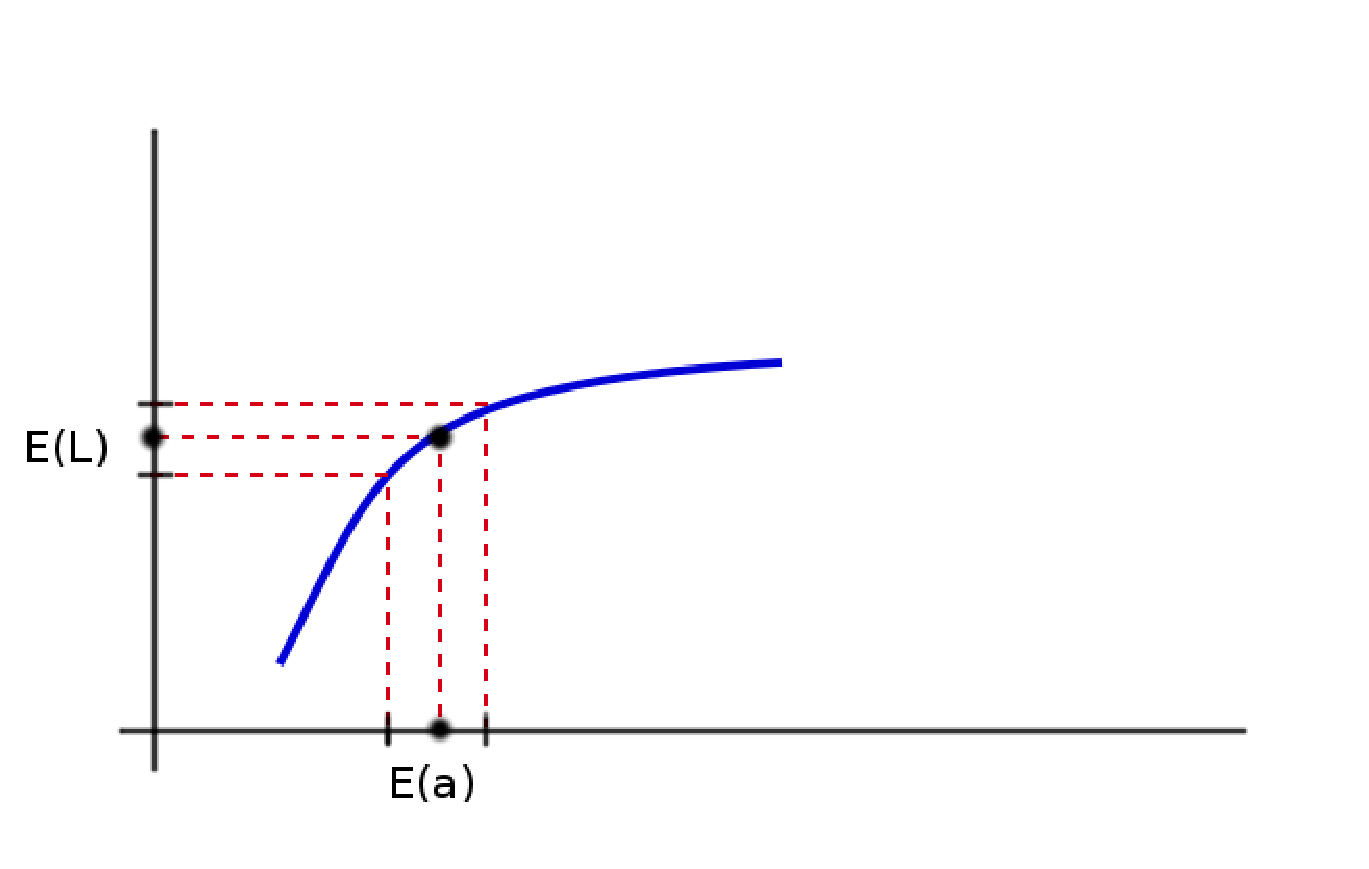
\includegraphics[height=6cm,width=6cm]{limite01.eps}
\end{center} 
\end{minipage}
\begin{minipage}{.50\textwidth}
Continuando...\\

Decimos que el limite de la funcion f cuando $x$ tiende a $a$ ($x$ se acerca a $a$) es igual a $L$ y se nota:
	$$ \lim_{x \rightarrow a}{f(x)} = L $$
\end{minipage}
\hfill \\\\
$\odot$ La fucnion $f$ deve estar al menos definida en $\stackrel{\circ}{E}(L)$\\
$\odot$ $E(L)$ depende de $E(a)$\\

Para poder trabajar se utiliza la siguiente definicion formal:

$$ \lim_{x \rightarrow a}{f(x)} = L   \Leftrightarrow   \forall \varepsilon >0, \exists \delta (\varepsilon) >0 /  0 < |x-a|< \delta \Leftarrow |f(x) - L| < \varepsilon $$

Esto es: El limite de $f(x)$ con $x$ tendiendo a $a$ es $L$ si y solo si  para todo $\varepsilon$ positivo, existe un $\delta$ en fucnion de $\varepsilon$ tal que el entorno reducido de centro $a$ y radio $\delta$ implicque que el valor absoluto de la resta de $f(x)$ menos $L$ sea menor a $\varepsilon$.\\

En si plantea que si evaluamos $f(x)$ en puntos cercanos a $a$, la funcion devolvera valores cercanos a $L$ que estaran edentro del entorno $E(L)$.

\subsubsection{Ejemplo de limite sensillo}
$$\lim_{x\rightarrow 2}{2x +1 =7}$$
Demostraremos eso:
$$ \forall \varepsilon > 0, \exists \delta (\varepsilon) >0 / 0<|x-3|<\delta \Rightarrow |(2x+1)- 7|<\varepsilon$$
Dado un $\varepsilon > 0$ (fijamos un $\varepsilon$ para poder trabajar).

$$ |(2x+1)-7| < \varepsilon \Rightarrow |2x+1-7| < \varepsilon \Rightarrow\ |2 \times (x-3)|< \varepsilon \Rightarrow 2 \times \underbrace{|x-3|}_{< \delta}< \varepsilon $$
$$ |x-3|< \delta \Rightarrow 2\delta < \varepsilon \Rightarrow \delta = \frac{\varepsilon}{2}$$
$\therefore$ Dado $\varepsilon>0, \exists \delta= \frac{\varepsilon}{2}$ tal que:
\begin{center}
$0<|x-3| < \frac{\varepsilon}{2} \Rightarrow 2(x-3)< \varepsilon       $  $ $ \checkmark demostrado.
\end{center}

\subsubsection{Pincipio de arquimedes}

Cada segmento ($y$) tan largo como se quiera puede ser cubiertos con un numero finito ($n$) de segmentos de longitud positiva tan pequenios como se quiera ($x$).
\begin{center}
\begin{pspicture}(0,0)(10,0.4)
\psaxes[labels=none]{-}(7,0)
\psdot(0.3,0)\rput[255](0.3,0.3){$x$}
\rput[255](0,-0.3){$0$}
\psdot(4,0)\rput[255](4,0.3){$y$}
\psdot(4.2,0)\rput[255](4.2,-0.4){$\overbrace{x\times n}$} 
\end{pspicture}\\ 
\end{center}

$$0<x<y<x\times n$$

\paragraph{Propiedad}
	Si tres nuemros reales $x$,$y$,$a$ satisfacen.
		$$ a \leq x \leq a + \frac{y}{n}  \forall n \in \mathbb{N}; x,y,a \in \mathbb{R}$$
		$$\therefore x=a$$
\subparagraph{Demostracion}

Hip: $a\geq 0$, $x>0$, $y>0$, $n>0$

Sup: $a<x$, $x>0$, $x-a>0$

Usando el principio de arquimedes, $x=x-a>0$
\begin{center}
$n\times (x-a)>y \Rightarrow x-a > \frac{y}{n} \Rightarrow $\\
$\Rightarrow x>a+\frac{y}{n} \leftarrow ABSURDO!!$\\
(Ya que $ a\leq a + \frac{y}{n}$)\\
\end{center}

Llegando a un absurdo mostramos que la supocicion es falsa($a<x$), por tanto deve ser $a=x$. 

\subsection{Unicidad de limite}

$$\lim_{x\rightarrow a}{f(x)}=L1 \wedge \lim_{x\rightarrow a}{f(x)}=L2 \Rightarrow L1=L2$$
\paragraph{Demostracion}

Hip:

• $\lim_{x \rightarrow a}{f(x)}=L1 \Leftrightarrow \forall \varepsilon >0, \exists \delta _1 (\varepsilon) / 0<|x-a|<\delta _1 \Rightarrow |f(x)-L1|<\varepsilon$

• $\lim_{x \rightarrow a}{f(x)}=L2 \Leftrightarrow \forall \varepsilon >0, \exists \delta _2 (\varepsilon) / 0<|x-a|<\delta _2 \Rightarrow |f(x)-L2|<\varepsilon$\\

Si tomamos un $\delta = \min {\delta _1, \delta _2}$ entonces nos queda:

Dado un $\varepsilon>0$, $\delta$
$$0<|x-a|<\delta \Rightarrow |f(x)-L1|<\varepsilon \wedge |f(x)-L2|<\varepsilon$$
\begin{center}
\fbox{
$a>0$, $b>0$, $c>0$ $\in \mathbb{R} \Rightarrow
\left.
\begin{array}{ccc}
a &<& c\\
b &<& c\\
\end{array}\right\} \Rightarrow a+b < c+c$}
\end{center}
$$\Rightarrow |f(x)-L1|+|f(x)-L2| < \varepsilon + \varepsilon \Rightarrow |f(x)-L1|-|f(x)-L2|<|f(x)-L1|+|f(x)-L2|< 2\varepsilon \Rightarrow$$
$$\Rightarrow |f(x)-L1-(f(x)-L2)|<2\varepsilon \Rightarrow |f(x)-L1-(f(x)-L2)|<2\varepsilon \Rightarrow$$
$$\Rightarrow |f(x)-L1- f(x)+L2|< 2\varepsilon \Rightarrow |L2-L1|< 2\varepsilon$$

En base a la propiedad del \textbf{Pincipio de Arquimedes}.
\begin{center}
\fbox{$a\leq x\leq a+ \frac{y}{n} \Rightarrow a=x$, donde $a$, $x$, $y$ $\in \mathbb{R}$ y $n \in \mathbb{N}$}
\end{center}

Tomando $a=0$, $x=|L2-L1|$, $\varepsilon=\frac{1}{2n}$ resulta:
$$0\leq |L2-L1|\leq 0+ 2\times \frac{1}{2n} \Rightarrow 0\leq |l2-l1|\leq \frac{1}{n} \Rightarrow 0=|L2-L1|\Rightarrow 0=L2-L1 \Rightarrow L2=L1 $$
\begin{center}
Son el mismo limite!
\end{center}

\subsection{Caracter local de limite}

Sean $f$ y $g$ dos funciones definidas en un $\stackrel{\circ}{E}(a)$ de manera que $\exists \delta >0 /$ \\ $ f(x)=g(x), \forall x/0<|x-a|<\delta$ entonces los limites de $f(x)$ y $g(x)$ con $x\rightarrow a$ son el mismo.

\paragraph{Demostracion} 


$$\lim_{x\rightarrow a}{f(x)}=L \Leftrightarrow \forall \varepsilon>0, \exists \delta _1 (\varepsilon)>0/0<|x-a|< \delta _1 \Rightarrow |f(x)-L|\varepsilon$$

Como por hipotesis $f(x)=g(x)$ $\forall x\in \stackrel{\circ}{E}(a,\delta _1)$. Tomo el minimo: $\delta _2 = \min {\delta _1 , \delta}$ ($\delta$ hipotesis).

Seguimos, dado $\varepsilon>0, \exists \delta _2/$
$$0<|x-a|\delta _2 \Rightarrow |f(x)-L|< \varepsilon \stackrel{\stackrel{en 0<|x-a|<\delta _2}{f(x)=g(x)}}{\Rightarrow} |g(x)-L<\varepsilon$$

Entonces dado $\varepsilon, \exists \delta _2 $
$$/ 0<|x-a|<\delta _2 \Rightarrow |g(x)-L|<\varepsilon \Leftrightarrow \lim_{x \rightarrow a}{g(x)}=L$$

$$\therefore \lim_{x \rightarrow a}{f(x)}=L =\lim_{x \rightarrow a}{g(x)}$$

\subsection{Formulas equivalentes}

\paragraph{1)}
$$\lim_{x \to a}{f(x)}=L \Leftrightarrow \lim_{x \to a}{f(x)-L}=0 \Leftrightarrow \lim_{x \to a}{|f(x)-L|}=0$$
 
\subparagraph{Demostracion \\}

$$\lim_{x \to a}{f(x)} =L\Leftrightarrow \forall \varepsilon >0, \exists \delta (\varepsilon)>0/ 0<|x-a|<\delta \Rightarrow |f(x)-L|<\varepsilon \Leftrightarrow$$
$$\Leftrightarrow 0<|x-a|<\delta \Rightarrow |f(x)-L|=|(f(x)-L)-0| <\varepsilon \Leftrightarrow \lim_{x \to a}{f(x)-L}=0 \Leftrightarrow$$
\fbox{$||x||=|x|$(propiedade de valor absoluto)}
$$\Leftrightarrow 0<|x-a|<\delta \Rightarrow |f(x)-L|=||(f(x)-L)-0|| <\varepsilon \Leftrightarrow \lim_{x \to a}{f(x)-L} = 0 $$

\paragraph{2) "Cambio de variable"}

$$\lim_{x \to a}{f(x)}=L \Leftrightarrow \lim_{h \to 0}{f(a+h)-L}=0 $$

\subparagraph{Demostracion \\ }

$$ \lim_{x \to a}{f(x)}=L \Leftrightarrow \forall \varepsilon >0, \exists \delta(\varepsilon)>0 / 0<|x-a|<\delta \Leftarrow |f(x)-L|< \varepsilon \Leftrightarrow$$
\begin{center}
  Defino $h=x-a$, $h=h-0$, despejo $x=a+h$ y sustituyo en la formula original quedando:
\end{center}
$$\Leftrightarrow 0<|h-0|<\delta \Leftarrow |f(a+h)-L| < \varepsilon \Leftrightarrow \lim_{h \to 0 }{f(a+h)}=L$$

\subsection{Teorema: "funcion acotada"}

Sea una funcion $f(x)$ con limite $L$ y vale $m<L<M$ entonces existe $\delta$ tal que $x\in \stackrel{\circ}{E}(a)$, $f(x)$ estara acotada inferiormente por $m$ y superiormente por $M$.

$$\lim_{x \to a}{f(x)}=L \wedge m<L<M \Rightarrow [\exists \delta >0/0<|x-a|<\delta \Rightarrow m<f(x)<M]$$

\paragraph{Demostracion \\}

Supuesto: $\lim_{x \to a}{f(x)}=L \wedge m<L<M$





\end{document}
